% !TEX TS-program = xelatex
% !BIB program = biber
% !TEX encoding = UTF-8 Unicode

% 使用手冊請見 TW_Thesis_Template wiki:
% https://github.com/sppmg/TW_Thesis_Template/wiki

% User guide in wiki of TW_Thesis_Template :
% https://github.com/sppmg/TW_Thesis_Template/wiki

\documentclass[]{NTHU_thesis} % \documentclass[option1, option2, ...]
% Helpful options: 
% draft = Don't load figure ,reduce compile time.
% showframe = show document margins.
% colorgrid = show colored coordinate. (by eso-pic pkg.)
\usepackage[subpreambles]{standalone} % standalone class setting in config.tex
% Option ``subpreambles'' enable sub-tex's preambles when compile main tex. (pkg default disable)
% sppmg think it's still some problem (e.g. \addbibresource will faild ), recommend move all subpreambles to ``macros_preamble.tex``

\begin{document}
    \frontmatter
        \startWatermark         % 由此開始每頁浮水印
        \documentclass[class=NTHU_thesis, crop=false, float=true]{standalone}
\begin{document}
% I use LaTeX3 to automatically generate name table. 
% Below \ExplSyntaxOn to \ExplSyntaxOff perpare prof. table contents,
% it will save contents to `\profsTableContent''. 
% You can ignore this block even you want make table by yourself.
\ExplSyntaxOn
% Copy prof. list from config.tex
\clist_gclear_new:N \g_sppmg_profsZh_cl
\clist_gset:NV \g_sppmg_profsZh_cl \profsZh
\clist_gclear_new:N \g_sppmg_profsEn_cl
\clist_gset:NV \g_sppmg_profsEn_cl \profsEn

% get total number of prof. . Omitted language will not display.
\int_gzero_new:N \g_sppmg_profTotal_int
\int_gset:Nn \g_sppmg_profTotal_int {
    \int_max:nn {\clist_count:N \g_sppmg_profsZh_cl} 
        {\clist_count:N \g_sppmg_profsEn_cl}
}

% NOTE: ``tabularx'' will  processes its contents more than once 
% for calculate width, so ``gpop'' can't put in tabularx env.
% \tl_if_exist:NTF {\tl_clear:N \g_sppmg_tableContent_tl} {\tl_new:N \g_sppmg_tableContent_tl}
% \tl_if_exist:NTF \g_sppmg_tableContent_tl {} {\tl_new:N \g_sppmg_tableContent_tl}
\tl_gclear_new:N \g_sppmg_tableContent_tl


% Use a inline function for pop 2 list (zh+en), and save table content 
% Input(#1) switch 3 case, 1 = Advisor, 2 = committee member , 3+ is more.
% Use ``for'' loop to get all prof.
\int_step_inline:nnnn {1}{1}{\g_sppmg_profTotal_int}{
    \clist_gpop:NNTF \g_sppmg_profsZh_cl \l_tmpa_tl {}{ \tl_clear:N \l_tmpa_tl}
    \clist_gpop:NNTF \g_sppmg_profsEn_cl \l_tmpb_tl {}{ \tl_clear:N \l_tmpb_tl}
    \tl_gput_right:Nx \g_sppmg_tableContent_tl {
        \int_case:nnTF {#1}{
            {1} {指導教授: & \l_tmpa_tl & 博士 & (Prof.~ \l_tmpb_tl ) \exp_not:n {\\} }
            {2} {共同指導: & \l_tmpa_tl & 博士 & (Prof.~ \l_tmpb_tl ) \exp_not:n {\\} }
        }{}{
            & \l_tmpa_tl & 博士 & (Prof.~ \l_tmpb_tl ) \exp_not:n {\\} 
        }
    }
}

% Copy contents to LaTeX2e macro.
\cs_set_eq:NN \profsTableContent \g_sppmg_tableContent_tl

\ExplSyntaxOff
\def\fsUniversity{\fs{24}[1.5]}
\def\fsTitle{\fs{20}[1.5]}
\def\fsNames{\fs{18}[1.5]}

\def\mcShift{\hspace{-6.0pt}} % It's for align non-multicolumn cell .
% --------define title page layout for thesis
\titlepageFontFamily % set in config.tex
\newgeometry{top=2.5cm, bottom=2.5cm, inner=2cm, outer=2cm} % only for titlepage
\begin{spacing}{1.0}
\begin{titlepage}
    \null\vfill
    \begin{center}
        {\fsUniversity 國\quad 立\quad 清\quad 華\quad 大\quad 學} \par
        \vspace*{5mm}
        
        {\fsTitle {\degree}論文\par}
        \vspace*{20mm}
        
        {\fsTitle {\title} \par}
        \vspace*{5mm}
        
        {\fsTitle {\subtitle} \par}
        \vspace*{10mm}
        
        {\ifx \logo\empty\vspace*{30mm}
        \else \includegraphics[height=30mm]{\logo} \par
        \fi}
        \vfill
        
        {\fsNames \renewcommand{\arraystretch}{1}
            % If you want make table by yourself, replace ``\profsTableContent''
            \begin{tabular}{l@{\hspace*{0.4em}}l@{\quad}l@{\quad}l}
            系\qquad 所: & \multicolumn{3}{l}{\mcShift \dept}      \\
            學\qquad 號: & \multicolumn{3}{l}{\mcShift \studentID} \\
            研\enspace 究\enspace 生: & \authorZh & & (\authorEn)    \\
            
            \profsTableContent
            
            \end{tabular}
        \par}
        \vspace*{5ex}
        
        {\fsTitle {\degreedate} \par}
        \vspace*{2ex}
        
        \ifthenelse{\boolean{printcopyright}}
        {{{版權所有\copyright\ \author\ \quad \copyyear} \par}}
        {}
    \end{center}
    \null\vfill
\end{titlepage}
\end{spacing}
\restoregeometry
\normalfont % use main font
%--------end of title page for thesis
\cleardoublepage
\end{document}
       % 封面/書名頁
        \listoftodos   % todo list, hide when set \textbackslash{}setboolean\{publish\}\{\textbf{true}\} in config.tex. It will not add to TOC , you can add \todototoc before \listoftodos to do that.
            \todoInfo{explain transverse}
            \todoInfo{abbreviation}
            \todoInfo{eta, phi, R definition}
            \todoInfo{add the study introduction in Chapter 1}
            \todoInfo{add references}
            \todoInfo{reproduce the feynman diagrams (not anti-q)}
            \todoUnsure{Unsure}
            \todoChange{Change}
            \todoInfo{Information}
            \todo[inline]{Inline}
            \missingfigure{Big Warning}

        %%%%%%%%%%%% letters %%%%%%%%%%%%
        % Set file name in config.tex
        % 依校方規定,此處須插入:
        % [v] 清大(電子授權書) 必備,不論是否授權都要裝訂
        % [v] 清大(紙本授權書) 必備,不論是否授權都要裝訂
        % [x] 國家圖書館(電子授權書) 有授權才要裝訂
        % [v] 國家圖書館(紙本論文延後公開/下架申請書)→紙本論文有申請延後公開才要裝訂
        % [v] 指導教授推薦書
        % [v] 考試委員審定書
        % !!! [x] 部份請自行插入

        % 碩博士論文電子檔授權書 Authorization Letter (for electronic)
        \IfFileExists{\letterAuthEl}{
            \cleardoublepage        % 由下個右頁開始
            \includepdf{\letterAuthEl}}{}
        % 碩博士論文紙本授權書 Authorization Letter (for paper)
        \IfFileExists{\letterAuthPa}{
            \cleardoublepage        % 由下個右頁開始
            \includepdf{\letterAuthPa}}{}
        % 國家圖書館(電子授權書) 有授權才要裝訂

        % 碩博士紙本論文延後公開/下架申請書。(如需延後公開者,才需要裝訂於論文內頁)
        \IfFileExists{\letterPubReq}{
            \cleardoublepage
            \includepdf{\letterPubReq}}{}
        % 指導教授推薦書
        \IfFileExists{\letterRecom}{
            \cleardoublepage
            \includepdf{\letterRecom}}{}
        % 口試委員審定書
        \IfFileExists{\letterVerif}{
            \cleardoublepage
            \includepdf{\letterVerif}}{}
        \cleardoublepage
        
        %%%%%%%%%%%% Other frontmatter, eg,abstract %%%%%%%%%%%%
        % 中英文論文摘要:內容應說明研究目的,資料來源,研究方法及研究結果等
        \documentclass[class=NTHU_thesis, crop=false]{standalone}
\begin{document}
\setlength{\parindent}{2em} %縮排2字寬

\chapter{摘要}
在利用衰變成一對底夸克對的希格斯粒子,來尋找與其相伴產生$Z^\prime$-2HDM模型的暗物質分析中,最後的擬合使用了$Z$玻色子衰變成兩個輕子的分布,來估計$Z$玻色子衰變成兩個微中子的背景。在過去的分析中是以舊有的分布比例當作參數,而在本論文中使用了最新的蒙地卡羅樣本衰變比例以增進分析結果。

\vspace{2em}
\noindent \textbf{關鍵字:} \keywordsZh{} % Set keywords in config.tex
\end{document} % zh 中文摘要
        \documentclass[class=NTHU_thesis, crop=false]{standalone}
\begin{document}

\chapter{Abstract}
In the search for the dark matter of the $Z^\prime$-2HDM model produced in association with a Higgs boson decaying to $b\bar{b}$, the kinematics of $Z \to ll$ are used to estimate $Z \to \nu\nu$, the main background of the process in the post-fit stage. Instead of using the ratio of the $Z \to \nu\nu$ decay channel to $Z \to ll$ decay channel based on the previous analysis, this thesis presents the improvement of the analysis by using the ratio of the updated Monte-Carlo (MC) samples of the $Z$ boson.

\vspace{2em}
\noindent \textbf{Keywords:} \keywordsEn{} % Set keywords in config.tex
\end{document} % en 英文摘要
        \documentclass[class=NTHU_thesis, crop=false]{standalone}
\begin{document}

\chapter{Acknowledgements}
感謝指導教授徐百嫻教授的辛勤指導。這段時間如沐春風,教授仰之彌高,鑽之彌堅。
\newline

感謝Patrick Rieck博士和Samuel Meehan博士給我這份難得可貴的機會,讓我參與這個分析。
\newline

感謝Philipp Gadow博士與呂昀儒博士,當我在程式編碼上遇到困難時,給了我大量的協助。
\newline

感謝韓正忻以及組內的其他人,是這份論文的分析一路下來的工作搭檔。
\newline

最後感謝媽媽全力支持,即使我的人生規劃和她所預期的有些出入。

\end{document}


 % 誌謝(可略)

        % 原始 book class 不將 TOC,LOF,LOT 加入目錄列表,須手動加
        % 此樣板可由 config.tex 切換是否自動加入目錄
        \tableofcontents        % 目錄
        \listoffigures          % 圖目錄
        \listoftables           % 表目錄
        \documentclass[class=NTHU_thesis, crop=false]{standalone}
\begin{document}

\chapter{Glossary}
Use table for symbol list. You can also use package ``nomencl'' (simple) or ``glossaries'' (powerful). see packages document or my tutorial (but it's Chinese).

\begin{table}[h]
    \normalsize
    \centering
    \begin{tabular}{c@{\quad:\quad}l}
%         Symbol  & Description \\ 
        VIM     & The best guy's editor \\ 
        Emacs   & The God's editor \\ 
        CTAN    & Comprehensive TeX Archive Network, ctan.org \\
        
    \end{tabular} 
    \caption*{Glossary} % Hide caption by comment/remove it, label will inactive also. 不想顯示請註解/刪除\caption行(\label自動失效)
    \label{table:glossary_def}
\end{table}

\end{document}
    % 符號說明
    \mainmatter
        \documentclass[class=NTHU_thesis, crop=false]{standalone}
\begin{document}


\chapter{Introduction}
In the universe, the galaxies are observed to violate Newton's second law with the rotation of the observable matters which is faster than expected. Thus it is thought that there are invisible matters called Dark Matter (DM) generating additional gravity to accelerate the rotation. The most popular hypothesis is proposed that DM is a stable and electrically natural particle $\chi$ which only has weak and gravitational interaction with the Standard Model (SM) particles. Thanks to the characteristics, we can try to search such particle at the Large Hadron Collider (LHC).

One possible model of DM is a Type-II two-Higgs-doublet model (2HDM) with an additional U(1)$_{Z^\prime}$ gauge symmetry, known as the $Z^\prime$-2HDM model. A light scalar $h$, which is identified as the SM Higgs boson, and a pseudo-scalar $A$ are introduced among this model, together with a striking process shown in \cref{fig:DM-Model}. The process has the attribute targeted by the collider searches that the final state is DM following with a detectable particle, the SM Higgs boson $h$ in this case. Due to the single visible Higgs boson in the final state, the search for DM of $Z^\prime$-2HDM model is called the monoH analysis. This analysis exploits the largest decay branching ratio of a Higgs boson into a pair of $b$-quarks.

\fig[0.45][fig:DM-Model][!hbt]{DM-Model.png}[The aimed process of the production of DM $\chi$ in the $Z^\prime$-2HDM model. A SM Higgs boson decaying to a pair of $b$-quarks is produced through a $Z^\prime$ mediator coupled to a pseudo-scalar Higgs boson $A$, which eventually decays to undetectable $\chi\bar{\chi}$.]

\end{document}    % 緒論
        \documentclass[class=NTHU_thesis, crop=false]{standalone}
\begin{document}

\chapter{ATLAS Detector}
\label{chap:ATLAS_Detector}
The ATLAS (A Toroidal LHC ApparatuS) \cite{1748-0221-3-08-S08003} is a multifunctional detector with a nominally forward-backward symmetric cylindrical geometry with respect to the interaction point. It comprises four detector components which are the inner detector tracking system, the electromagnetic (EM) calorimeter, the hadronic calorimeter and the muon spectrometer. The overview of the ATLAS is shown in \Cref{fig:ATLAS}.

\fig[0.7][fig:ATLAS][!hbt]{ATLAS.jpg}[The overview of the ATLAS.]

The inner detector is composed of three sub-detectors, the silicon pixel layers, the silicon microstrip (SCT) layers and the transition radiation tracker (TRT), shown in \Cref{fig:ID}. The silicon pixels and the SCT are placed in the range of $\left|\eta\right| < 2.5$, providing the information of pattern recognition, outstanding momentum resolution and both primary and secondary vertex measurements. The TRT comprises many layers of gaseous straw-tube tracking detectors in the range of $\left|\eta\right| < 2.0$, taking charge of continuous charged-particle tracks to improve the pattern recognition and enhance the momentum resolution and also giving the electron identification.

\fig[0.7][fig:ID][!hbt]{ID.jpg}[The schematic diagram of the ATLAS inner detector, which comprises three sub-components, pixels, SCT and TRT. Besides the three pixel layers shown in the figure, there is also a newly added layer, the Insertable B-Layer (IBL) \cite{Capeans:1291633}, as the innermost silicon pixel, improving the identification of displaced vertices and the $b$-tagging performance.]

The calorimeters measure electron, photon, jet and $\tau$ lepton energies, covering the range of $\left|\eta\right| < 4.9$, shown in \Cref{fig:Calorimeter}. The EM calorimeters are liquid argon (LAr) detectors which are accommodated in three cryostats, two end-caps and one barrel, covering the range of $\left|\eta\right| < 3.2$. The LAr is used because of its inherent behavior, stability of response over time and intrinsic radiation-hardness.

Outside the EM calorimeter envelope, the hadronic calorimeter can be divided into the LAr hadronic end-cap calorimeters, the LAr forward calorimeters and the tile calorimeters for the range of $\left|\eta\right| < 4.9$. The LAr hadronic end-cap calorimeters cover the range of $1.5 < \left|\eta\right| < 3.2$, sharing the cryostats with the EM end-cap calorimeters and the forward calorimeters. The LAr forward calorimeters are placed in the range of $3.1 < \left|\eta\right| < 4.9$. As mentioned previously, the LAr is chosen for its inherent excellent property. The tile calorimeters consist of one central barrel calorimeter and two extended barrel calorimeters, made of steel as the absorber and scintillating tiles as the active material, laying over the range of $\left|\eta\right| < 1.7$.

\fig[0.8][fig:Calorimeter][!hbt]{Calorimeter.jpg}[The schematic diagram of the calorimeters, composed of the EM calorimeter and the hadronic calorimeter.]

The outmost component is the muon spectrometer. Over the range of $\left|\eta\right| < 2.7$, the high-precision tracking chambers measure muon tracks in the large superconducting air-core toroid magnets. There are also the trigger chambers covering the range of $\left|\eta\right| < 2.4$ for providing bunch-crossing identification, providing well-defined $p_T$ thresholds, and measuring the muon coordinate in the direction orthogonal to that determined by the precision-tracking system.

The superconducting magnetic system is significantly featured in the ATLAS. As shown in \Cref{fig:ATLAS}, the magnet system consists of one solenoid magnet, one barrel toroid magnet and two end-cap toroid magnets. The solenoid magnet gives $2\, \mathrm{T}$ magnetic field for the inner detector, bending the tracks of charged particles for the momentum measurement and minimizing the radiative density in front of the barrel EM calorimeter. The barrel toroid magnet and the end-cap toroid magnets produce a $0.5\, \mathrm{T}$ and $1\, \mathrm{T}$ toroidal magnetic field in the central and end-cap regions respectively, supplying the bending power for the muon detectors.

Because of the cylindrical structure, all the directional physical quantities used in the analysis are transverse. Apart from the azimuthal angle $\phi$ and the angle between the momentum and the the beam axis $\theta$, some geometrical variables are also defined. The pseudorapidity $\eta$ describes the angle of a particle relative to the beam axis, defined as $\eta = -\ln[\tan(\theta/2)]$. In addition, the rapidity $R$ is used for a measure of angular separation between particles, defined as $R = \sqrt{(\Delta\eta)^2 + (\Delta\phi)^2}$.

Apart from the detector structure, there are also the trigger system carrying out the event selection. There are up to one billion proton-proton collisions per second in the ATLAS and the trigger system only selects 100 events worth retaining per second. There are three levels for the selection process. The Level-1 trigger searches for high $p_T$ muons, electrons, photons, jets, $\tau$ leptons and large missing and total transverse energy. The Level-2 trigger tags these events with some specific regions of interest, leaving below 3500 events per second. In the end, approximately 200 events after the Level-3 trigger.
\end{document}          % 分析方法
        \documentclass[class=NTHU_thesis, crop=false]{standalone}
\begin{document}

\chapter{Background Estimation Strategy}
\label{chap:estimation_strategy}
As shown in \Cref{fig:DM-Model}, the signature of the DM model is large transverse missing energy with two $b$-quarks. Some SM processes show the same signature, becoming the background in the analysis. The main background processes of the analysis are $Z$($\nu\nu$) + jets, $W$($l\nu$) + jets and $t\bar{t}$, shown in \Cref{fig:Bkg-Processes}. In the $Z$($\nu\nu$) + jets process, the undetectable neutrinos in the final state are regarded as the missing energy. Thus once the jets are tagged as $b$-jets, the case will be background. In the $W$($l\nu$) + jets and $t\bar{t}$ processes, once the lepton is misidentified as the missing energy, the procedure will be interference as well.

\begin{figure}[!hbt]
	\captionsetup[subfigure]{labelformat=empty}
	\centering
	\subcaptionbox
	{$Z$($\nu\nu$) + jets
		\label{fig:Bkg-Processes-fig1}}
		{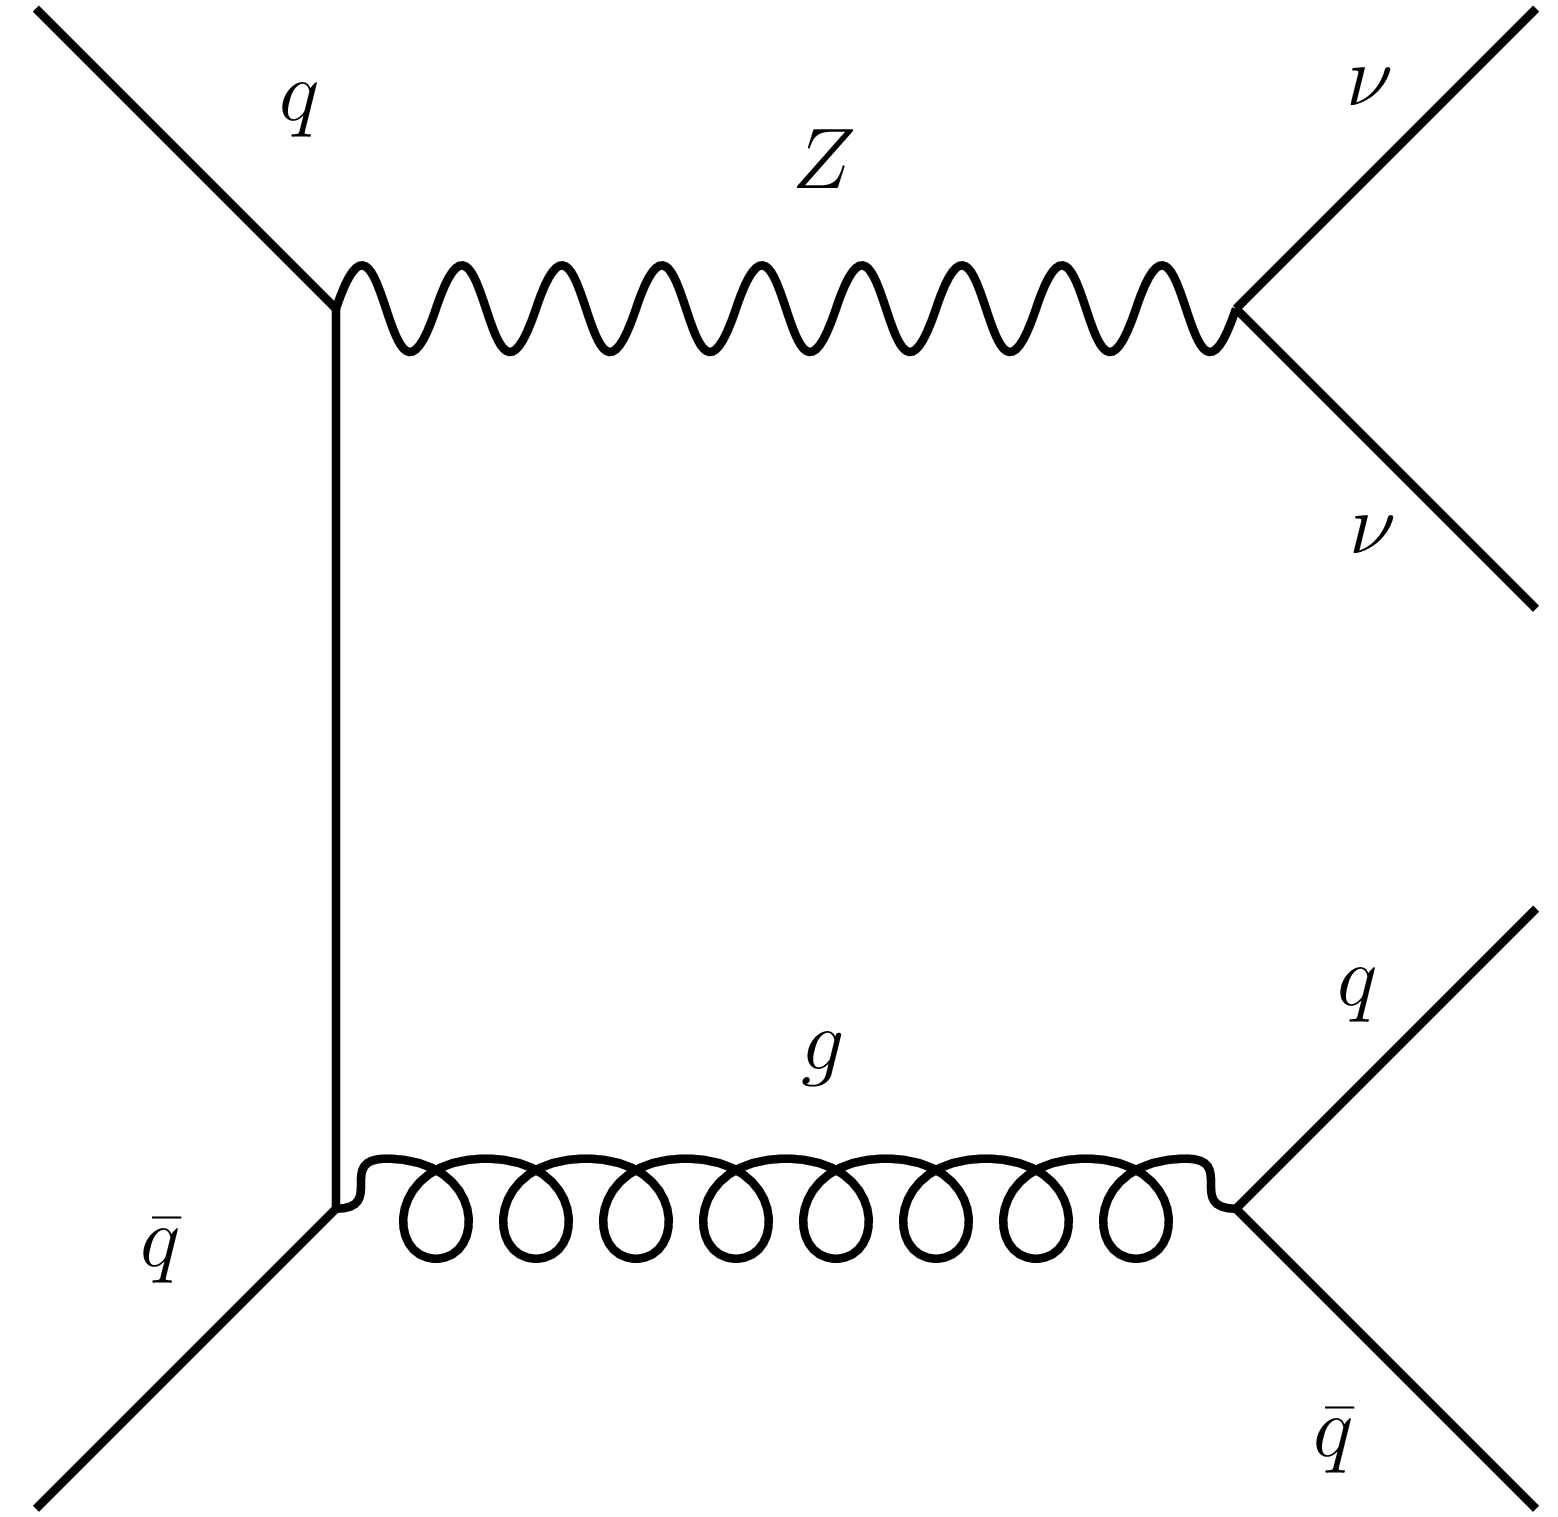
\includegraphics[width=0.32\linewidth]{Zvv.png}}
	\subcaptionbox
	{$W$($l\nu$) + jets
		\label{fig:Bkg-Processes-fig2}}
		{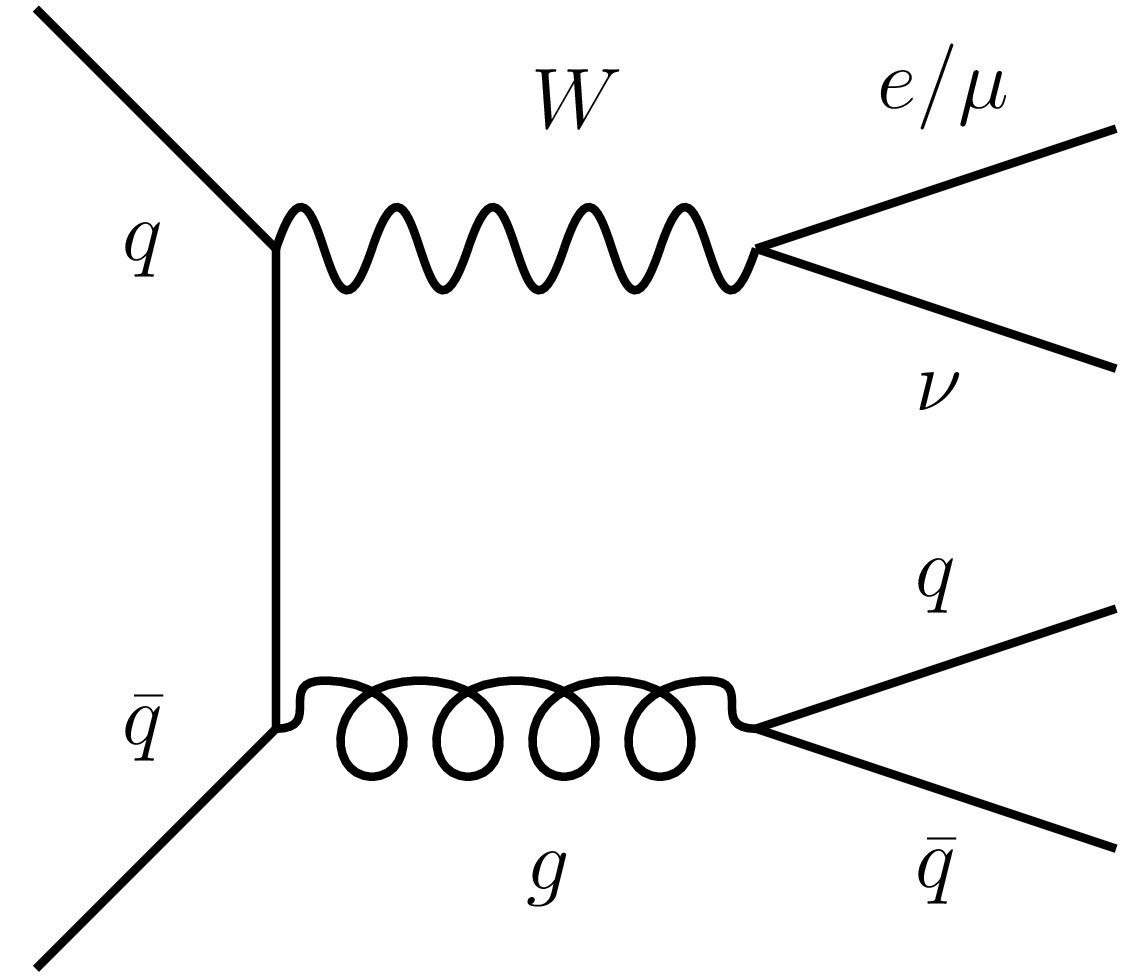
\includegraphics[width=0.32\linewidth]{Wlv.png}}
	\subcaptionbox
	{$t\bar{t}$
		\label{fig:Bkg-Processes-fig3}}
		{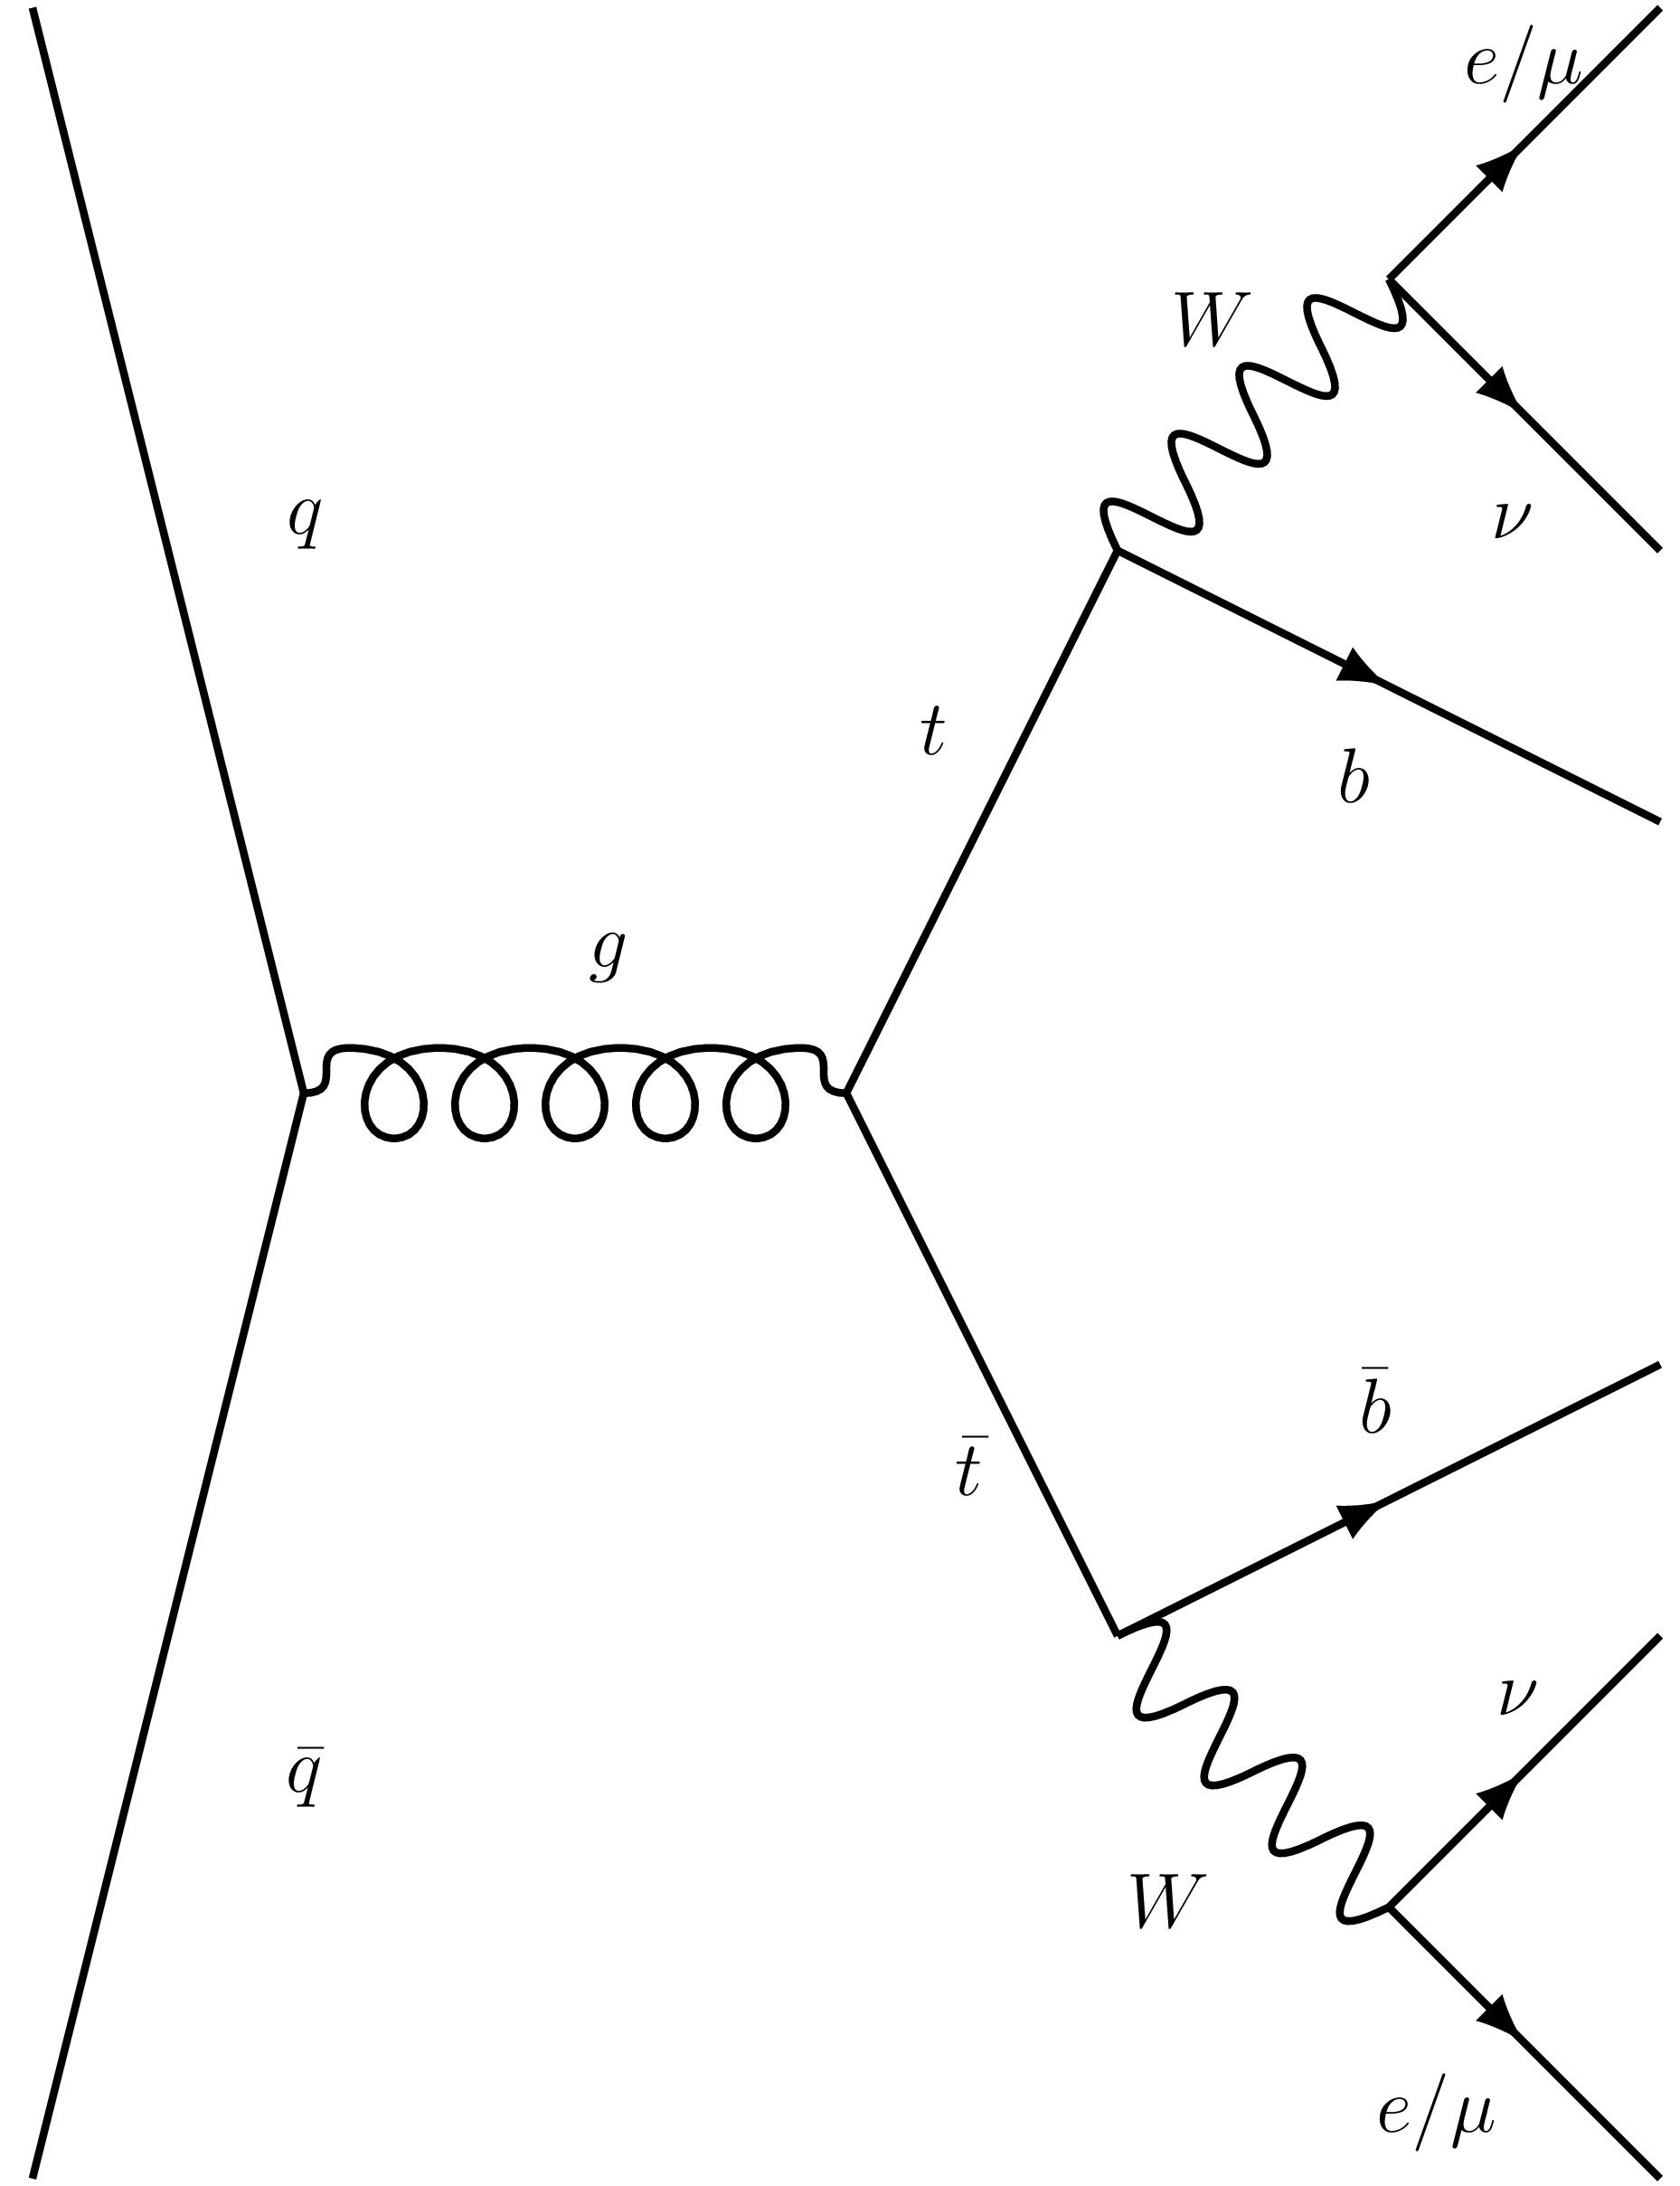
\includegraphics[width=0.32\linewidth]{ttbar.png}}
	\caption{The main background processes of the monoH analysis.}
	\label{fig:Bkg-Processes}
\end{figure}

To constrain the backgrounds, the control region (CR) strategy is used. Before defining the CR, the signal region (SR) is defined as where the signals are expected to show. The SR is required to have no lepton based on the model. Then the CR is defined as the orthogonal region to the SR. There are two CRs in this analysis, the one-muon CR and the two-lepton CR. The one-muon CR contains two processes, $W$($\mu\nu$) + jets and $t\bar{t}$, constraining $W$($l\nu$) + jets and $t\bar{t}$ in the SR. It requires different number of misidentified leptons, one in the SR but none in the one-muon CR. The two-lepton CR exploits the $Z$($ll$) + jets, constraining the $Z$($\nu\nu$) + jets process. Because it is not easy to simulate the misidentification as well as the kinematics of invisible neutrinos, these two CRs can constrain the background processes well.

\end{document}
        \documentclass[class=NTHU_thesis, crop=false]{standalone}
\begin{document}

\chapter{Object Reconstruction and Selection}
\label{chap:object_reconstruction}
\section{Jets}
Jets are a method to describe hadronic showers in detectors, consisting of multiple objects. Jets are reconstructed with the anti-$k_t$ algorithm\cite{1126-6708-2008-04-063}. Depending on the toplogical clusters, the radius parameter of $R = 0.4$ is the small-radius (small-$R$) jets and of $R = 1.0$ is the large-radius (large-$R$) jets.

The small-$R$ jets with $p_T > 20\, \mathrm{GeV}$ for $\left|\eta\right| < 2.5$ are regarded to as the central jets. The MV2c10 discriminant\cite{ATL-PHYS-PUB-2015-022} is used for $b$-tagging the central jets to identify the $b$-hadrons, with the 77\% efficiency. The efficiency is defined in the MC simulation as the ratio of the number of the $b$-tagged jets to the number of all jets with the truth value of $b$-jet. In addition, the small-$R$ jets with $p_T > 30\, \mathrm{GeV}$ for $2.5 < \left|\eta\right| < 4.5$ are the forward jets. The large-$R$ jets are required to have $p_T > 200\, \mathrm{GeV}$ and $\left|\eta\right| < 2.0$. The reconstructed topologies of the large-$R$ jets cover multiple constituent jets which are called the track jets. The track jets are linked to the large-$R$ jets with ghost association method\cite{1126-6708-2008-04-005}\cite{CACCIARI2008119}. The flavor identification for the large-$R$ jets depend on the ghost-associated track jets with the MV2c10 discriminant with the 77\% $b$-tagging efficiency. The track jets are described more in the following.

The fixed-radius (FR) track jets are applied for $b$-tagging in the previous analysis, using the anti-$k_t$ algorithm with fixed radius parameters. Instead of the FR track jets, the variable-radius (VR) track jets\cite{0903.0392} are implemented in the analysis for improving the $b$-tagging efficiency. The primary characteristic of the VR track jets is the relevance between the $p_T$ and the jet radius parameter: 
\begin{equation}
R \to R_{eff}(p_T) \approx \frac{\rho}{p_T}
\end{equation}
where $\rho$ is a constant factor.

\section{Leptons}
Electrons are reconstructed with energy deposits in the EM calorimeter which matches tracks in the ID. Besides the basic reconstruction, there are two types of electrons for the further selection in the analysis, the baseline electrons and the signal electrons. The baseline electrons have a loose criterion with $\left|\eta\right| < 2.47$ and $p_T > 7\, \mathrm{GeV}$, while the signal electrons require $\left|\eta\right| < 2.47$ and $p_T > 27\, \mathrm{GeV}$. The signal electrons are used to be tighter requirement for the regions requesting events to have electrons. The baseline electrons are used for other requirement about electrons, like electron vetoes.

The muon reconstruction relies on the muon spectrometer in the range of $\left|\eta\right| < 2.7$. It's also claimed to match the tracks in the ID for $\left|\eta\right| < 2.5$. Like electrons, there are two categories of muons, the baseline muons and the signal muons. The baseline muons is required to be with $\left|\eta\right| > 2.7$ and $p_T < 7\, \mathrm{GeV}$. The signal muons are defined with the criterion of $\left|\eta\right| < 2.5$ and $p_T > 25\, \mathrm{GeV}$. Same as the electrons, the signal muons are used to be the criterion for the region which needs events to hold muons, while the baseline muons are for other requirement conditions about muons.

Because of the hadronic-like nature of taus, the reconstruction is complicated and described in \cite{ATLAS-CONF-2017-029}. For the tau vetoes in the analysis, the taus are required to have one or three tracks and have $\left|\eta\right| < 2.5$ and $p_T > 20\, \mathrm{GeV}$, excluding the crack region $1.37 < \left|\eta\right| < 1.52$.

\section{Missing Transverse Momentum}
The missing transverse momentum is determined as the negative vector sum of the transverse momentum of all the reconstructed and calibrated objects in an event. Additionally, the track-based soft term is added into the missing transverse momentum in the analysis, which is from the tracks that not associated with any reconstructed object but still linked to the primary vertex. The absolute value of the missing transverse momentum is expressed as $E^{miss}_T$. Also, there is a purely track-based missing transverse momentum calculated as the negative vector sum of the transverse momentum of all the reconstructed tracks associated with the primary vertex. The absolute value of the track-based missing transverse momentum is denoted as $p^{miss}_T$.

Furthermore, to recognize whether the $E^{miss}_T$ is from weakly interacting particles or from the mis-measurement of multi-jet processes, two kinds of the $E^{miss}_T$ significance are applied. One is the event-based $E^{miss}_T$ significance defined as $E^{miss}_T/\sqrt{{\sum}p^{lepton}_T+{\sum}p^{jet}_T}$ and performed in the previous monoH analysis\cite{Meehan:2225941}, and the other is the object-based $E^{miss}_T$ significance which is newly introduced in the analysis, in order to reject multi-jet backgrounds. The object-based $E^{miss}_T$ significance is defined in \cite{ATLAS-CONF-2018-038}.

\end{document}
        \documentclass[class=NTHU_thesis, crop=false]{standalone}
\begin{document}

\chapter{Event Selection}
\label{chap:event_selection}
All the event data are from the proton-proton collision at $\sqrt{s} = 13\, \mathrm{TeV}$, recorded by the ATLAS detector during 2015, 2016 and 2017. Only data passed good operating conditions are used for the data quality. The integrated luminosity is $79.8 \pm 1.6\, \mathrm{fb}^{-1}$ in the analysis.

For different signal topology, the SR is divided into two parts, the resolved region ($E^{miss}_T < 500\, \mathrm{GeV}$) and the merged region ($E^{miss}_T > 500\, \mathrm{GeV}$). The small-$R$ jets consist the Higgs boson candidate in the resolved region, while the large-$R$ jets are expected to be the signature in the merged region. To estimate the backgrounds of the SR, the CRs are also divided into two divisions with the $p_T$ of the vector boson ($W$ or $Z$) as the separation boundary ($p^V_T < 500\, \mathrm{GeV}$ for the resolved region and $p^V_T > 500\, \mathrm{GeV}$ for the merged region). The event selection is different in the resolved region and the merged region. In the following, the common event selection is introduced before the selection for each region. In the end, the total event selection is summarized in \cref{table:summary_event_selection}.

\section{Common Selection}
The events have to pass the lowest un-prescaled triggers\cite{Lowest_un-prescaled_triggers}, and have at least one reconstructed vertex with at least two associated tracks with $p_T > 0.4\, \mathrm{GeV}$. To suppress the non-collision processes, the events are selected if $E^{miss}_T > 150\, \mathrm{GeV}$ in the SR and $p^V_T > 150\, \mathrm{GeV}$ in the CRs. Also, there are lepton requirements in each channel, no lepton in the SR, exactly one signal muon in the one-muon CR and two baseline leptons of which at least one is a signal lepton in the two-lepton CR. The events with tau leptons are vetoed. Moreover, in order to reduce the multi-jet processes, two conditions are applied. First, the azimuthal angular difference between $E^{miss}_T$ and the three highest small-$R$ jets (min$\Delta\phi(E^{miss}_T, jets_{1, 2, 3})$) is required to be larger than $20^\circ$. Second, the azimuthal angular difference between the direction of $E^{miss}_T$ and $p^{miss}_T$ ($\Delta\phi(E^{miss}_T, p^{miss}_T)$) is required to less than $90^\circ$. In addition, $H_T$ ratio cut\cite{Meehan:2225941} exploits the ratio of the $p_T$ of the Higgs boson candidates to $p_T$ of all jets, in order to reduce the $t\bar{t}$ background.

\section{Resolved Region}
The events are required to have at least two central small-$R$ jets. Exactly two of the jets are $b$-tagged and at least one of them have $p_T > 45\, \mathrm{GeV}$. The two $b$-tagged jets consist the Higgs boson candidate and their mass is required to be $50\, \mathrm{GeV} < m_{jj} < 280\, \mathrm{GeV}$. The scalar $p_T$ sum of first two (three) jets has to larger than $120 (150)\, \mathrm{GeV}$ for the events with two (three or more) jets. To further suppress the multi-jet background, the azimuthal difference between the Higgs boson candidate and $E^{miss}_T$ ($\Delta\phi(E^{miss}_T, h)$) is required to be larger than $120^\circ$. The azimuthal difference between the two jets which form the Higgs boson candidate ($\Delta\phi(jet_1, jet_2)$) is required to be less than $140^\circ$, and the ${\Delta}R$ between them to be less than $1.8$. In the SR and the one-muon CR, the object-based $E^{miss}_T$ significance is applied to be larger than $16$. Otherwise, the event-based $E^{miss}_T$ significance is applied to be less than $3.5\, \sqrt{\mathrm{GeV}}$ in the two-lepton CR.

\section{Merged Region}
It is required that to have at least one central large-$R$ jet of which the leading one is associated with two leading $b$-tagged VR track jets. The events with any $b$-tagged VR track jet outside the large-$R$ jet are vetoed. The large-$R$ jet is the Higgs boson candidate and the mass is required to be $50 < m_{J} < 270\, \mathrm{GeV}$.

\begin{table}[!h]
	\centering
	\begin{tabularx}{1\textwidth}{ |
			>{\setlength\hsize{1\hsize}\centering}X|>{\setlength\hsize{1\hsize}\centering}X| } 
		\hline
		Resolved Region  & Merged Region \tabularnewline
		\hline \hline
		\multicolumn{2}{|c|}{number of leptons = 0 (SR), 1 (one-muon CR), 2 (two-lepton CR)} \tabularnewline
		\hline
		\multicolumn{2}{|c|}{lowest un-prescaled triggers, vertex requirement} \tabularnewline
		\hline
		$150\, \mathrm{GeV} < E^{miss}_T$ (SR), $p^V_T$ (CRs) $ < 500\, \mathrm{GeV}$ & $E^{miss}_T$ (SR), $p^V_T$ (CRs) $ > 500\, \mathrm{GeV}$ \tabularnewline
		\hline
		\multicolumn{2}{|c|}{$\tau$-veto} \tabularnewline
		\hline
		\multicolumn{2}{|c|}{min$\Delta\phi(E^{miss}_T, jets_{1, 2, 3}) > 20^\circ$} \tabularnewline
		\hline
		\multicolumn{2}{|c|}{$\Delta\phi(E^{miss}_T, p^{miss}_T) < 90^\circ$} \tabularnewline
		\hline
		\multicolumn{2}{|c|}{$H_T$ ratio cut} \tabularnewline
		\hline
		number of central small-$R$ jets = 2 & number of central large-$R$ jets = 1 \tabularnewline
		\hline
		$p^{jet_1}_T > 45\, \mathrm{GeV} \parallel p^{jet_2}_T > 45\, \mathrm{GeV}$ & - \tabularnewline
		 \hline
		2 $b$-tagged small-$R$ jets & 2 $b$-tagged VR track jets \tabularnewline
		\hline
		$50\, \mathrm{GeV} < m_{jj} < 280\, \mathrm{GeV}$ & $50\, \mathrm{GeV} < m_{J} < 270\, \mathrm{GeV}$ \tabularnewline
		\hline
		$\sum_{i = 1}^{2(3)} p^{jet_i}_T > 120 (150)\, \mathrm{GeV}$ & - \tabularnewline
		\hline
		$\Delta\phi(E^{miss}_T, h) > 120^\circ$ & - \tabularnewline
		\hline
		$\Delta\phi(jet_1, jet_2) < 140^\circ$& - \tabularnewline
		\hline
		${\Delta}R < 1.8$ & - \tabularnewline
		\hline
		$E^{miss}_T$ significance cut& - \tabularnewline
		\hline
	\end{tabularx}
	\caption{The summary of the event selection.}
	\label{table:summary_event_selection}
\end{table}

\end{document}
        \documentclass[class=NTHU_thesis, crop=false]{standalone}
\begin{document}

\chapter{Systematic Uncertainties}
\label{chap:systematic_uncertainties}
In the analysis, the systematic uncertainties come from the reconstruction of physics objects and from theoretical predictions of both the signals and backgrounds. The dominant experimental systematic uncertainties originate from the $b$-tagging efficiency, which is mainly from the calibration of the flavor tagging efficiency of $t\bar{t}$ events \cite{ATL-PHYS-PUB-2017-013}. The experimental systematic uncertainties from the reconstruction of the $E^{miss}_T$, the leptons and the jets are obtained with the tools provided by the E/gamma, MCP and JetEtMiss combined performance group.

The theoretical systematic uncertainties are sourced from the modeling of the signal and the background processes, the MC statistics and the luminosity. The uncertainty of the modeling is from the processes of $V$ + jets, $t\bar{t}$, SM Higgs boson decaying to $b\bar{b}$ associated with a vector boson ($VH(bb)$) and diboson for the most part, which is derived in the SM $VH(bb)$ analysis \cite{Aaboud2017}. The estimate of the systematic uncertainties of the $V$ + jets, the biggest backgrounds, depend on two studies. One is varying the parameters of different MC generators to evaluate the acceptance uncertainties. The other is using data-driven shape comparisons in high purity regions, as described in \Cref{chap:Z_bkg_estimation}. Besides, the luminosity uncertainty is obtained from calibrations of the luminosity scale \cite{Aaboud2016}. The ranking of the dominant systematic uncertainties is shown in \Cref{table:uncertainty_ranking}, with the statistical uncertainty and the total uncertainty of the analysis.

\begin{table}[h]
	\centering
	\begin{tabular}{ l c c c }
		\hline
		\multirow{2}{*}{Source of uncertainty} & \multicolumn{3}{c}{Impact (\%)} \\ \cline{2-4}
		 & (a) & (b) & (c) \\ \hline
		$b$-tagging & 4.0 & 8.0 & 10 \\
		$V$ + jets modeling & 3.5 & 6.0 & 5.0 \\
		Top modeling & 3.7 & 4.8 & 4.5 \\
		MC statistics & 1.8 & 5.4 & 4.9 \\
		SM $Vh$($b\bar{b})$ & 0.8 & 3.2 & 2.1 \\
		Diboson modeling & 0.8 & 1.5 & 1.1 \\
		Signal modeling & 3.0 & 2.5 & 1.5 \\
		Luminosity & 2.0 & 2.5 & 2.5 \\
		Small-$R$ jets & 1.4 & 3.0 & 2.0 \\
		Large-$R$ jets & 0.2 & 1.0 & 2.0 \\
		$E^{miss}_T$ & 1.2 & 1.7 & 1.1 \\
		Leptons & 0.2 & 0.8 & 0.7 \\ \hline
		Total systematic uncertainties & 6.5 & 13 & 13 \\
		Statistical uncertainty & 2.3 & 20 & 23 \\
		Total uncertainty & 7 & 24 & 25 \\ \hline
	\end{tabular}
	\caption{The dominant source of the systematic uncertainties after the fit. Three representative sets of the parameters of $Z^\prime$-2HDM are shown: (a) $(m_{Z^\prime}, m_A) = (0.6\, \mathrm{TeV}, 0.3\, \mathrm{TeV})$, (b) $(m_{Z^\prime}, m_A) = (1.4\, \mathrm{TeV}, 0.6\, \mathrm{TeV})$ and (c) $(m_{Z^\prime}, m_A) = (2.6\, \mathrm{TeV}, 0.3\, \mathrm{TeV})$, assuming the total cross-sections of (a) $452\, \mathrm{fb}$, (b) $3.75\, \mathrm{fb}$ and (c) $2.03\, \mathrm{fb}$. The total uncertainty is the quadrature sum of the statistical and the total systematic uncertainties.}
	\label{table:uncertainty_ranking}
\end{table}

\end{document}
        \documentclass[class=NTHU_thesis, crop=false]{standalone}
\begin{document}


\chapter{Z Boson Background Estimation}
\label{chap:Z_bkg_estimation}
To estimate the $Z$($\nu\nu$) + jets background in the SR, the two-lepton CR is utilized with the fact that the momentum of $Z$ bosons doesn't rely on the decay result. After the event selection introduced in \Cref{chap:event_selection}, the pre-fit data versus MC distribution of the mass of the Higgs boson candidates $m_{bb}$ comparisons for the two-lepton CR are shown in \Cref{fig:2-lep-prefit}.

\begin{figure}[!hbt]
	\captionsetup[subfigure]{labelformat=empty}
	\centering
	\subcaptionbox
		{$150\, \mathrm{GeV} < p^V_T < 200\, \mathrm{GeV}$
		\label{fig:2-lep-prefit-fig1}}
		{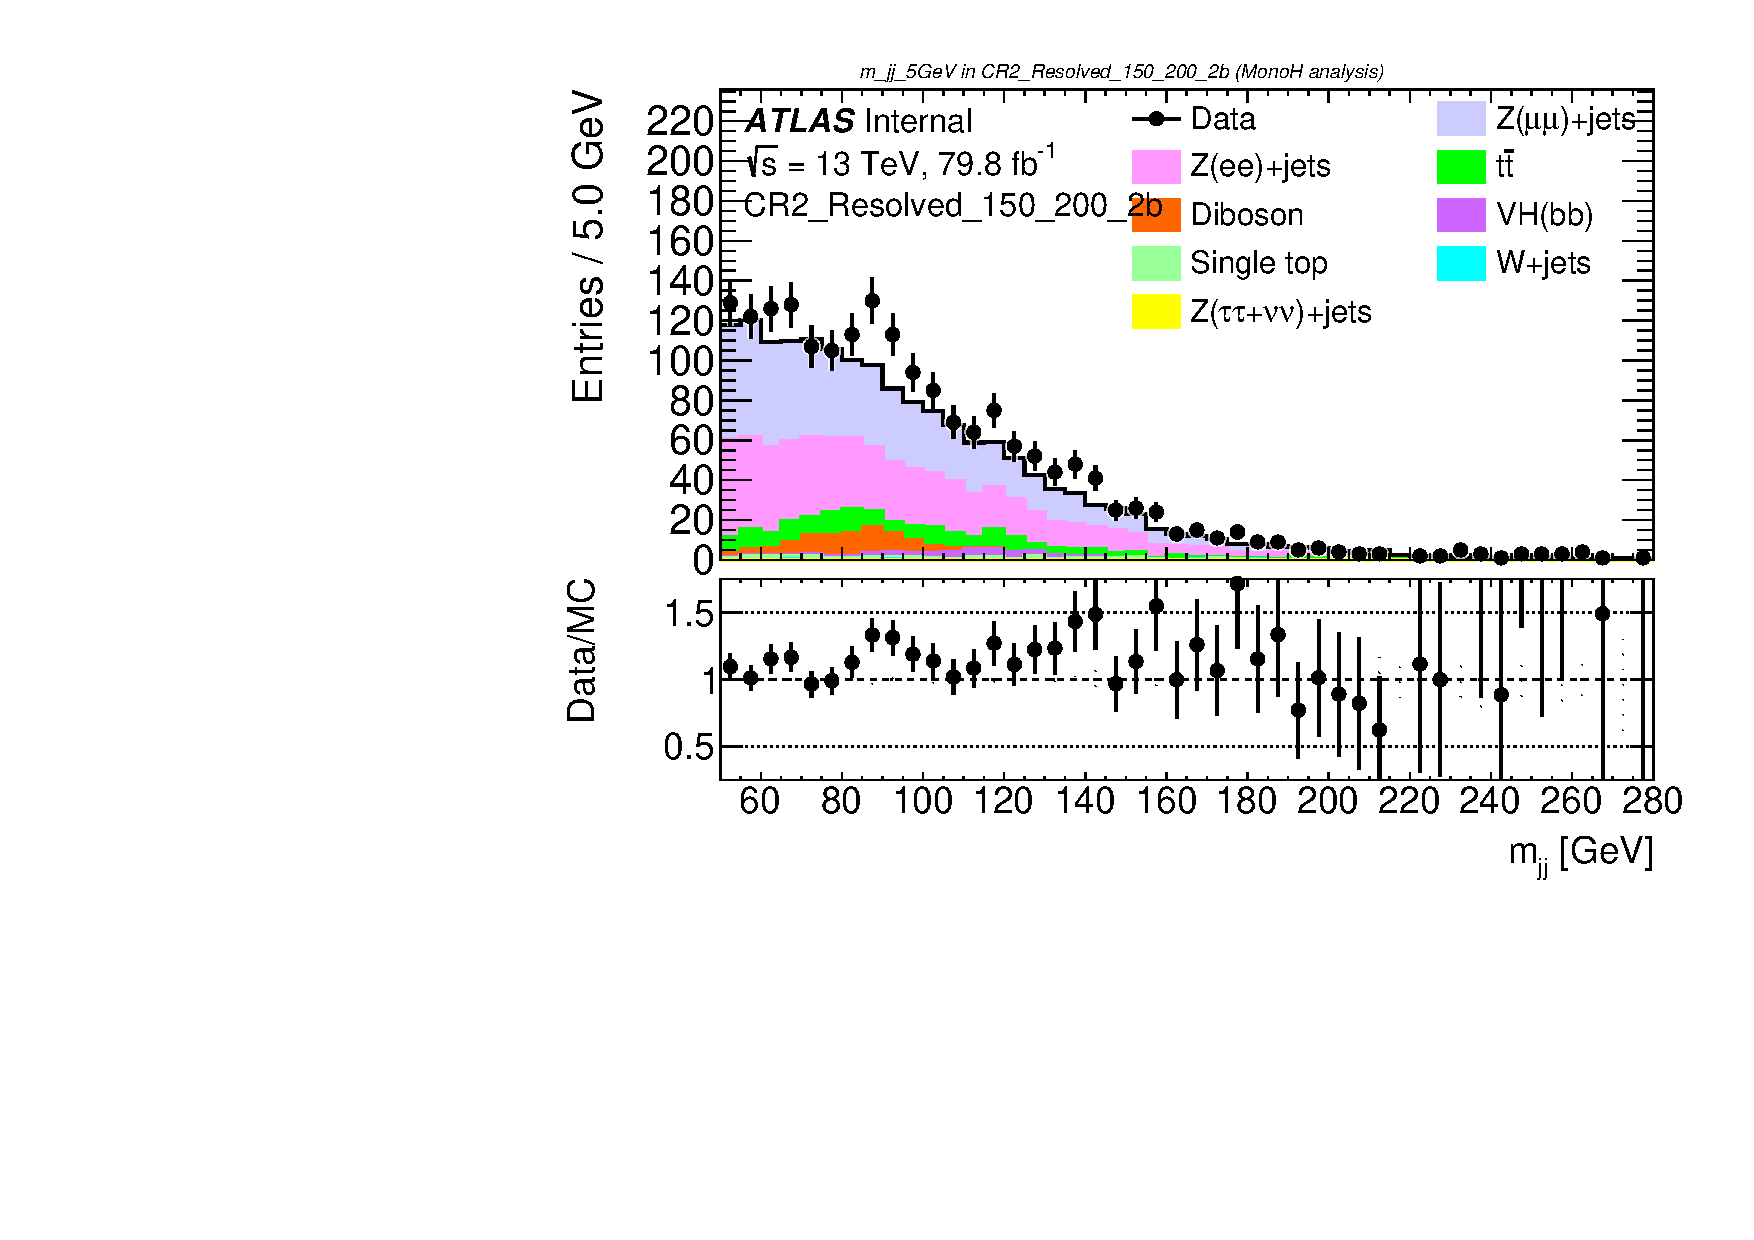
\includegraphics[width=0.47\linewidth]{prefit-150-200.pdf}}
	\subcaptionbox
		{$200\, \mathrm{GeV} < p^V_T < 350\, \mathrm{GeV}$
		\label{fig:2-lep-prefit-fig2}}
		{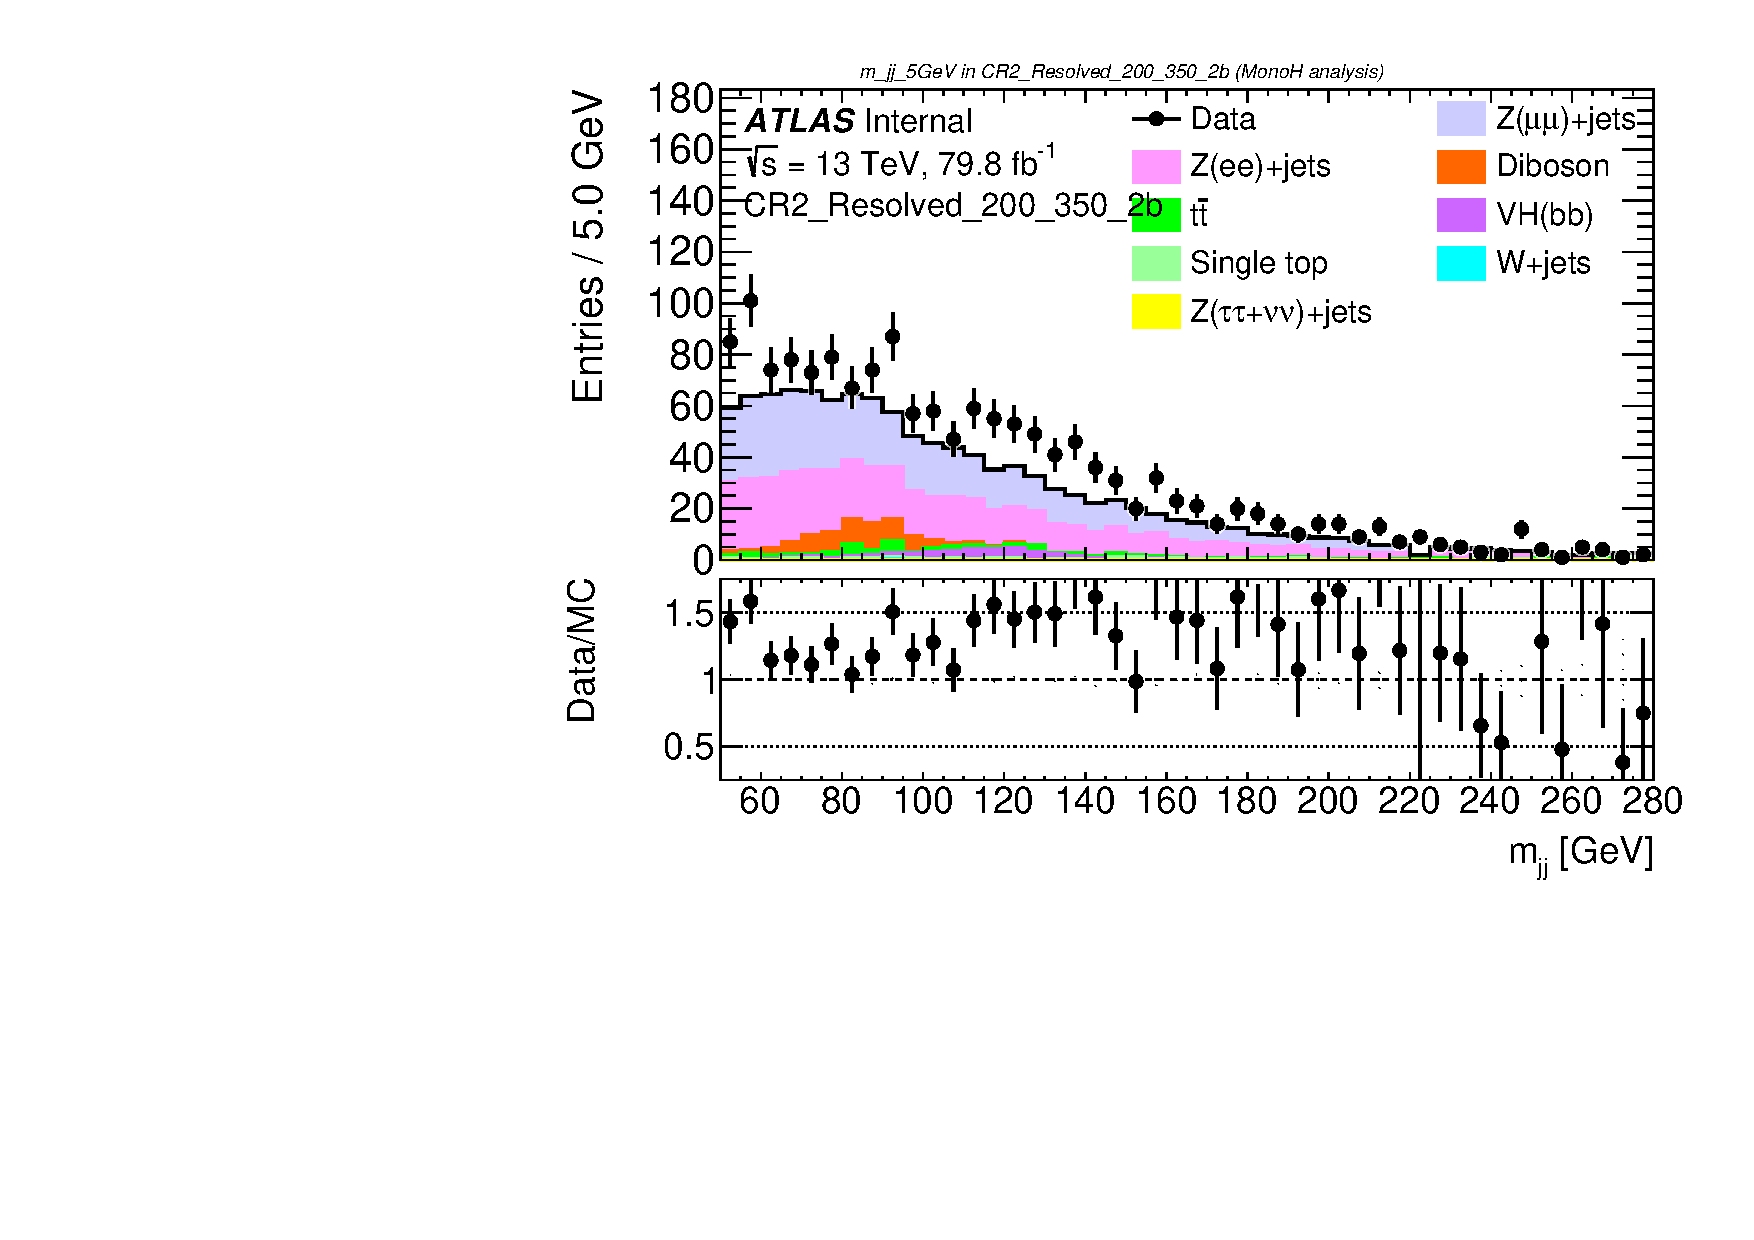
\includegraphics[width=0.47\linewidth]{prefit-200-350.pdf}}
	\vspace{\baselineskip}
	\subcaptionbox
		{$350\, \mathrm{GeV} < p^V_T < 500\, \mathrm{GeV}$
		\label{fig:2-lep-prefit-fig3}}
		{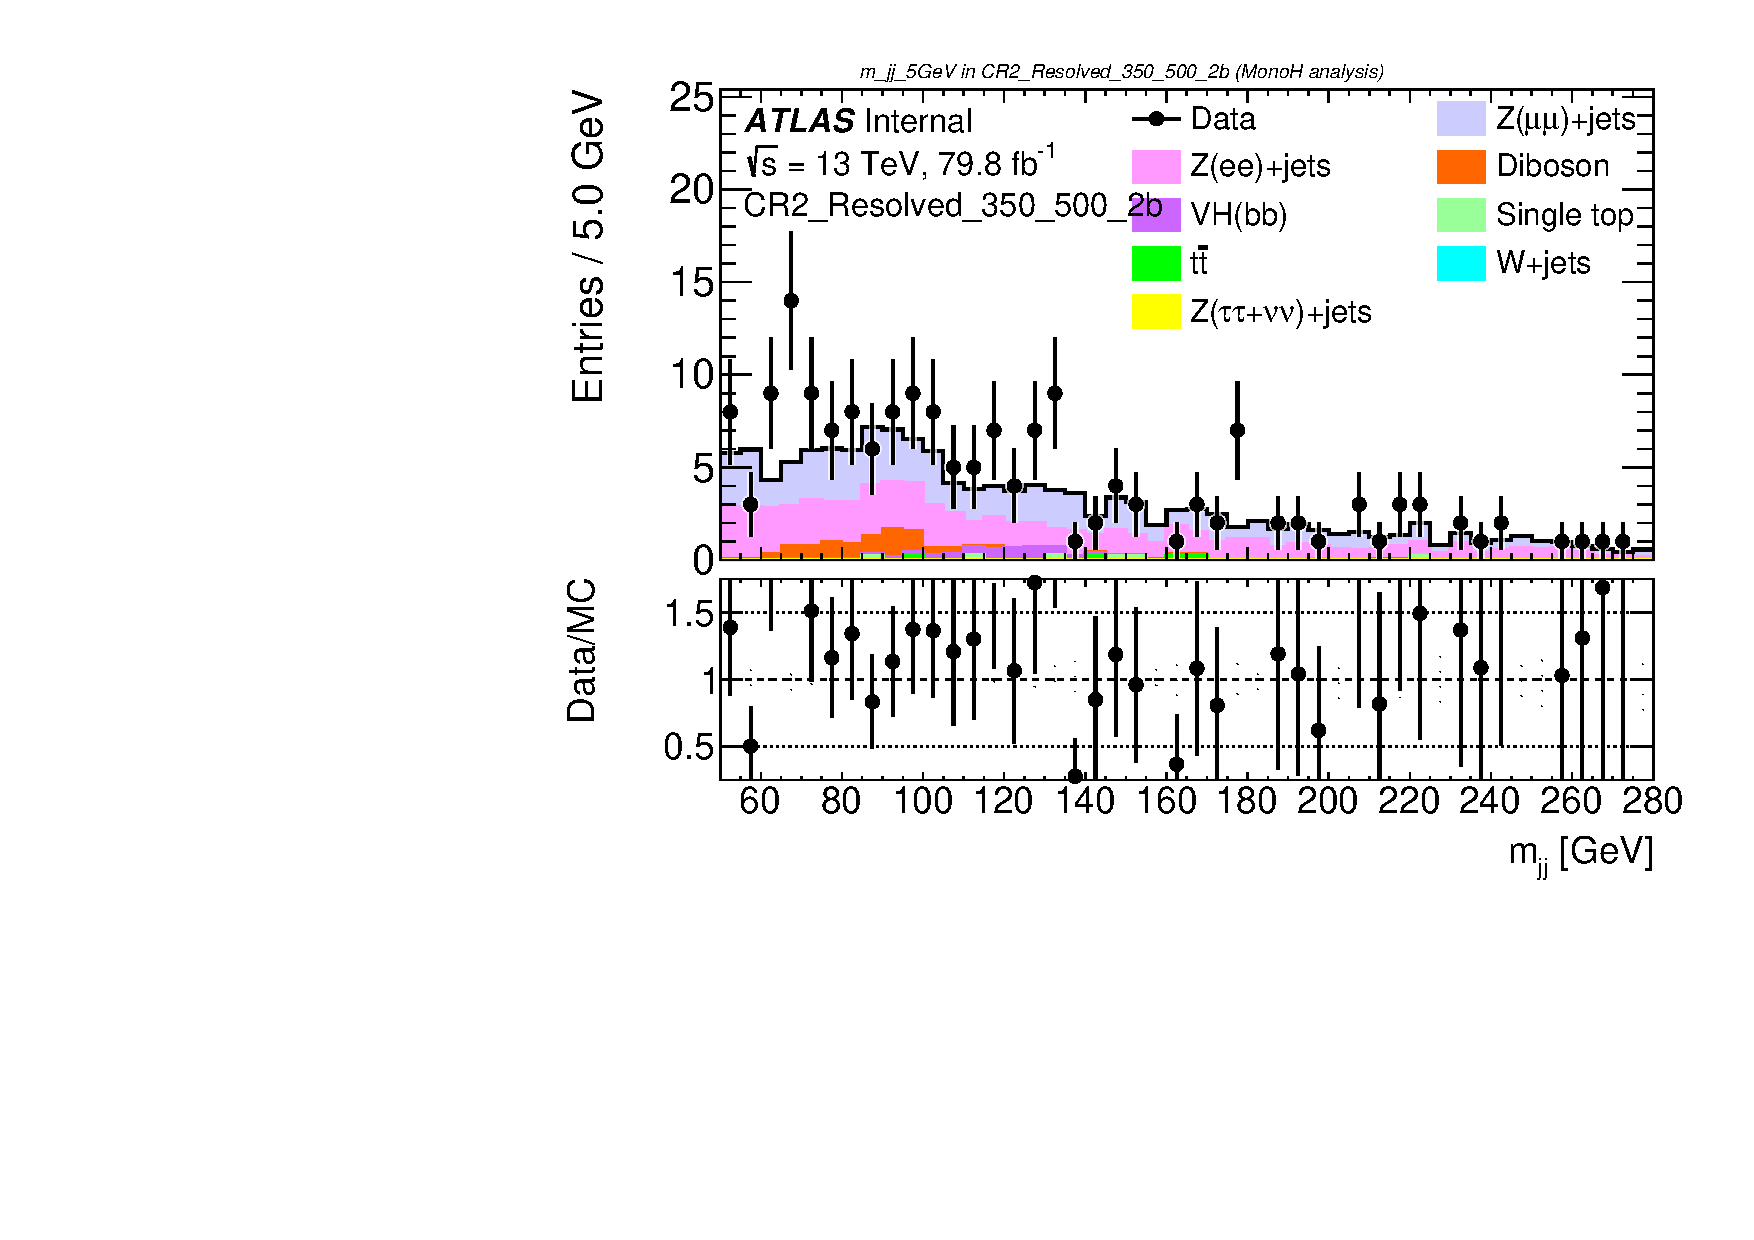
\includegraphics[width=0.47\linewidth]{prefit-350-500.pdf}}
	\subcaptionbox
		{$p^V_T > 500\, \mathrm{GeV}$
		\label{fig:2-lep-prefit-fig4}}
		{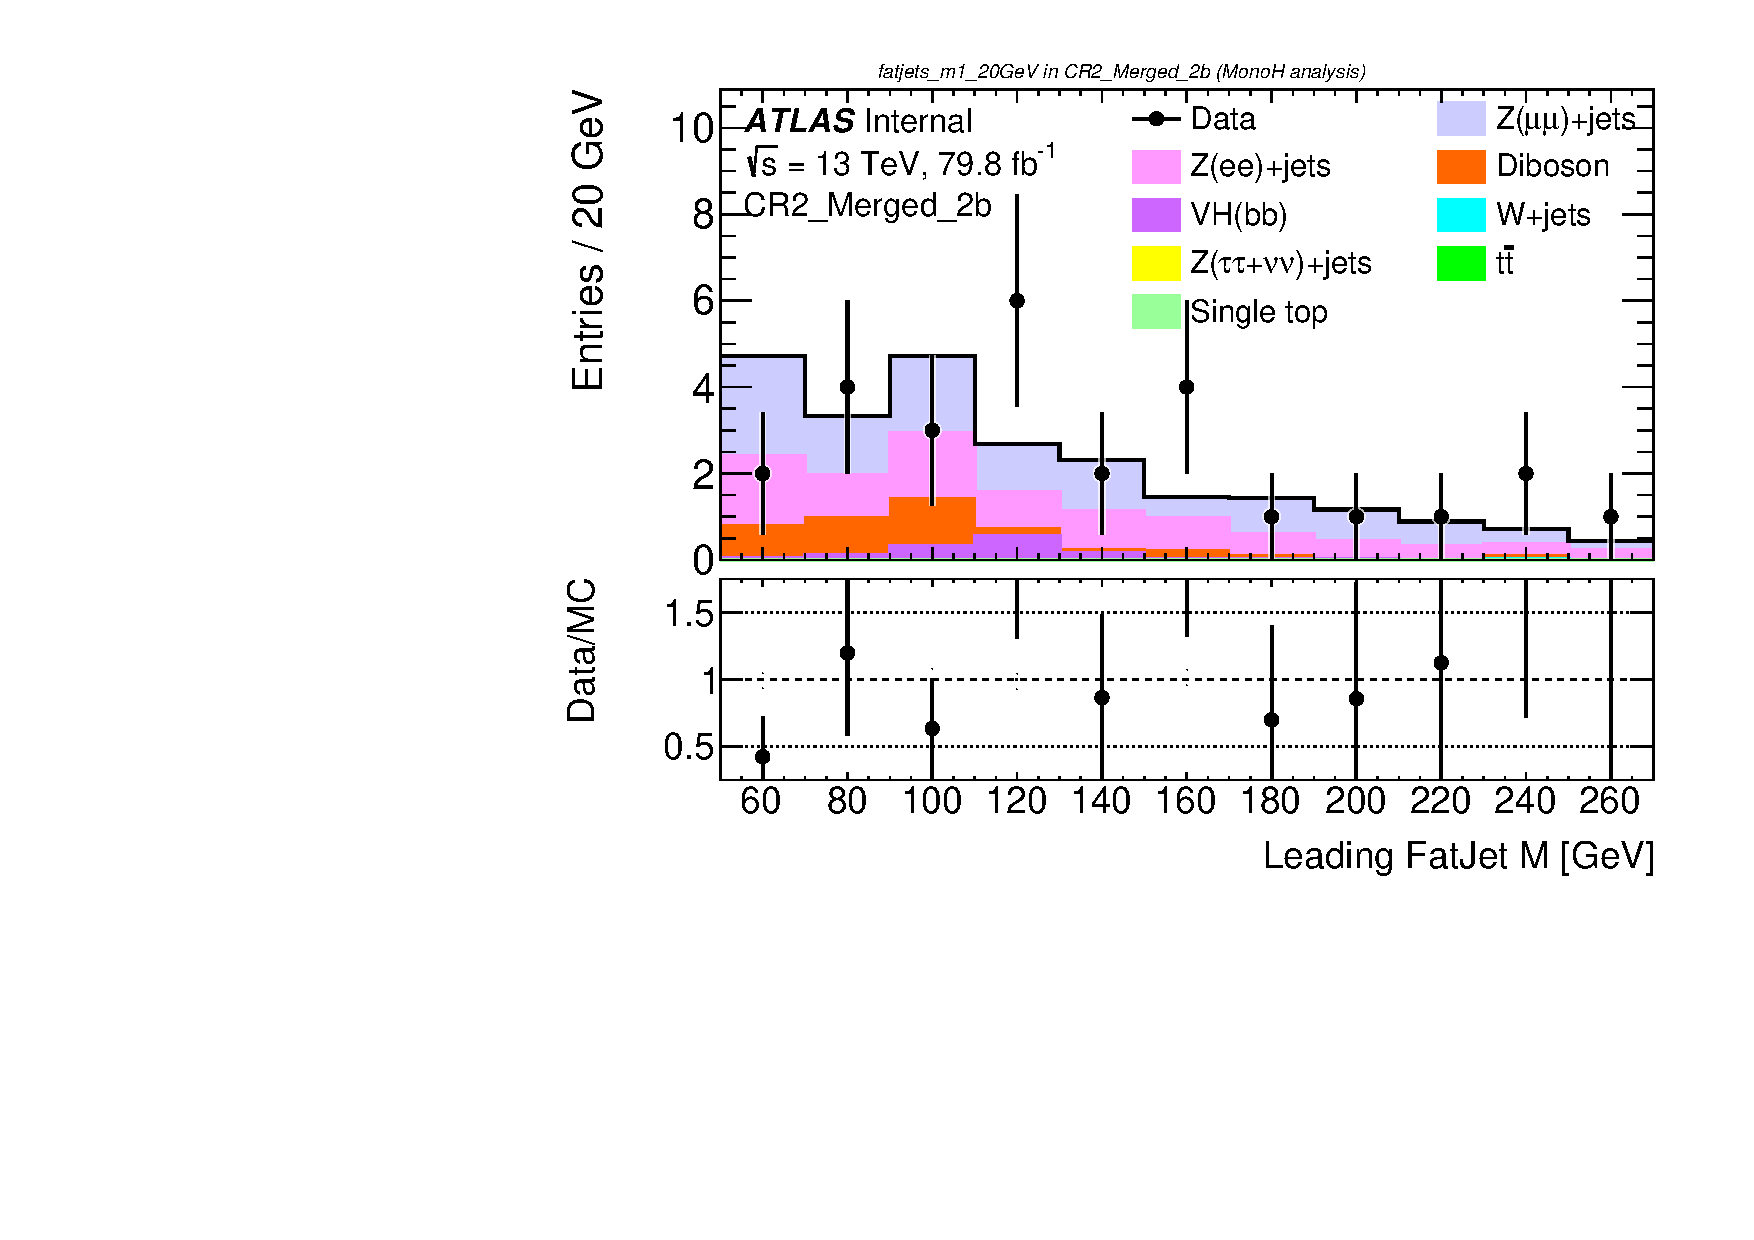
\includegraphics[width=0.47\linewidth]{prefit-500.pdf}}
	\caption{The pre-fit data/MC comparison of $m_{bb}$ distribution. The plots are split into four $p^V_T$ regions for fitting.}
	\label{fig:2-lep-prefit}
\end{figure}

The MC is compared to the data for the distribution for deriving the shape uncertainty in the two-lepton CR. Due to the high purity, the data-driven shape comparison is used for the estimation of the systematic uncertainty on the theoretical prediction of the $Z$ + jets modeling. The shape uncertainty is extracted by following the previous $VH$($bb$) analysis \cite{ATLAS-CONF-2018-036} and is used for two variables, $m_{bb}$ and $p^V_T$. To check if the functions can still give a reasonable estimation, the shape uncertainty and the normalized distribution of $m_{bb}$ and $p^V_T$ are shown in \Cref{fig:shape-uncertainty}. The distributions of the two variables are normalized and compared. The derived functions representing the shape uncertainty on $p^V_T$ and $m_{bb}$ are $\pm 0.2\, \mathrm{log}_{10} (p^V_T/50\, \mathrm{GeV})$ and $\pm 0.0005 (m_{jj} - 100\, \mathrm{GeV})$.

\begin{figure}[!hbt]
	% \captionsetup[subfigure]{labelformat=empty}
	\centering
	\subcaptionbox
	{The distribution of $m_{bb}$.
		\label{fig:shape-uncertainty-fig1}}
		{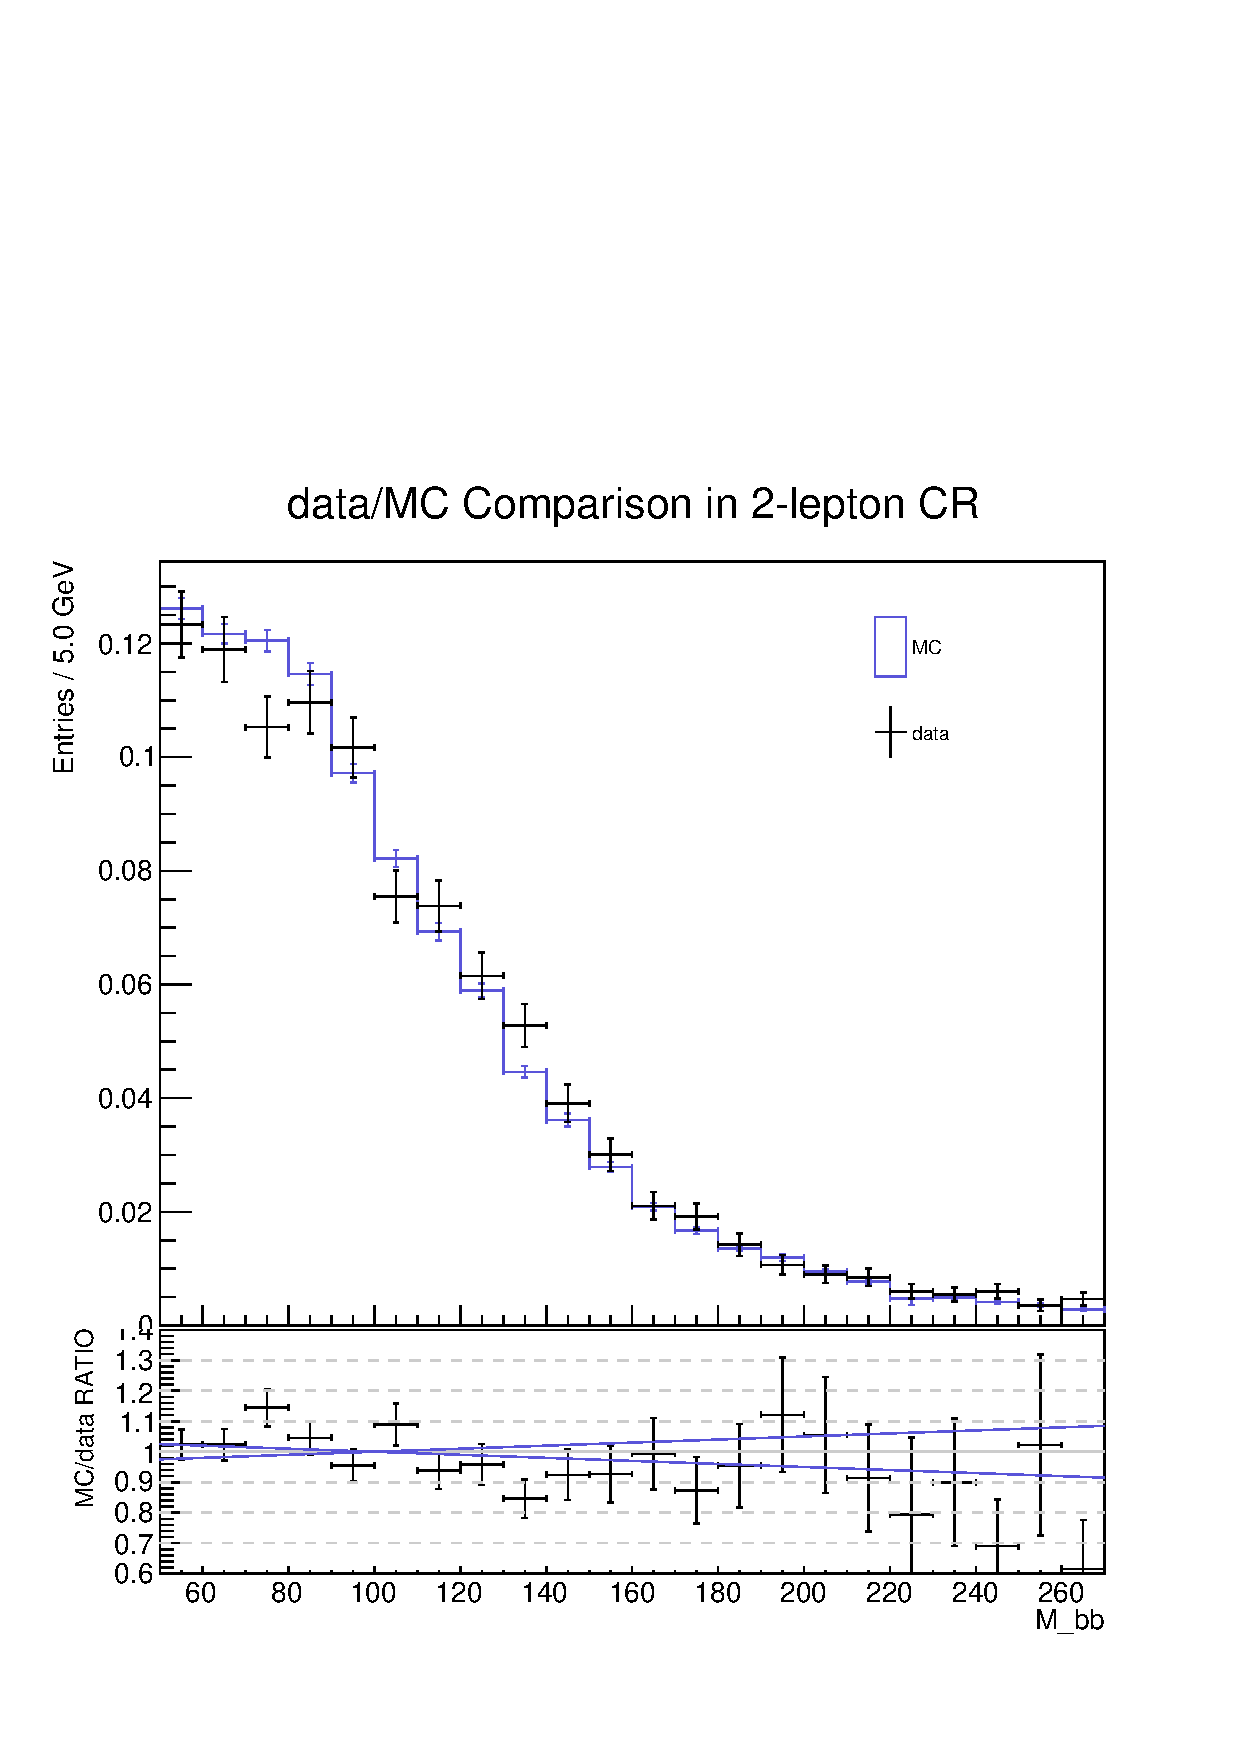
\includegraphics[width=0.65\linewidth]{shape-uncertainty-Mbb.pdf}}
	\vspace{\baselineskip}
	\subcaptionbox
	{The distribution of $p^V_T$.
		\label{fig:shape-uncertainty-fig2}}
		{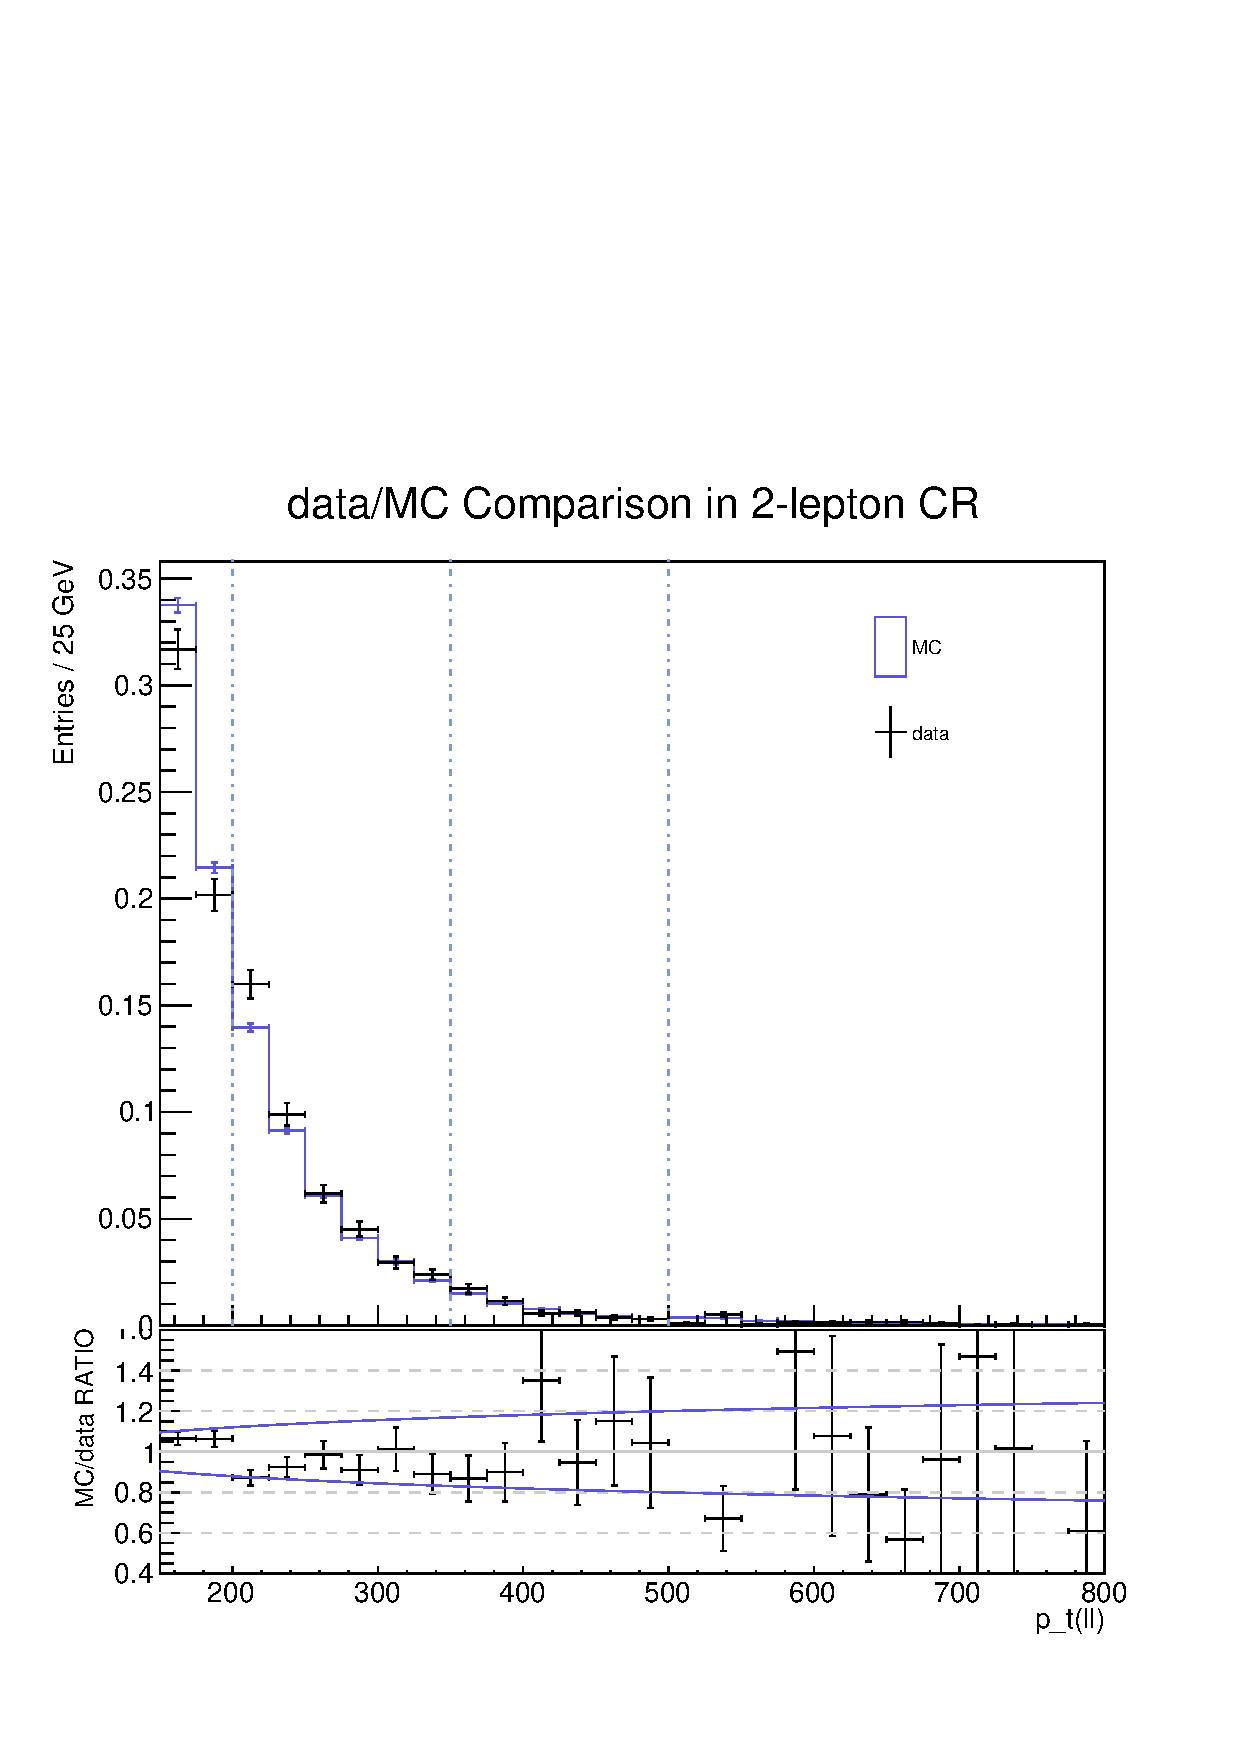
\includegraphics[width=0.65\linewidth]{shape-uncertainty-PTV.pdf}}
	\caption{The shape uncertainties and the normalized distributions of (a) $m_{bb}$ and (b) $p^V_T$. The shape uncertainties are derived by the $VH$($bb$) analysis and gives a reasonable estimation.}
	\label{fig:shape-uncertainty}
\end{figure}

To extrapolate the $Z$ + jets from the two-lepton CR to the SR, the distribution of $p^V_T$ of the $Z$($ll$) + jets and the $Z$($\nu\nu$) + jets are compared in \Cref{fig:Zvv-vs-Zll}. An uncertainty is applied as the decorrelation in the SR due to the larger purity of the $Z$ + jets prediction in the two-lepton CR. This uncertainty is set to be 7\% by following the $VH$($bb$) analysis \cite{ATLAS-CONF-2018-036} and gives a reasonable estimation in the resolved region. For the merged region, this uncertainty doesn't work so well because the merged region concept is not used in the $VH$($bb$) analysis. In the end, the post-fit results are presented in \Cref{fig:2-lep-postfit}. The normalization factor is extracted in the fit and used for the $Z$($\nu\nu$) + jets background in the SR, which is described in the \Cref{chap:result}.

\fig[0.65][fig:Zvv-vs-Zll][!hbt]{Zvv-vs-Zll.pdf}[The comparison of the normalized distributions of the $Z$($ll$) + jets and the $Z$($\nu\nu$) + jets. The uncertainty of the extrapolation from the two-lepton CR to the SR is 7\%, derived by the previous $VH$($bb$) analysis.]

\begin{figure}[!hbt]
	\captionsetup[subfigure]{labelformat=empty}
	\centering
	\subcaptionbox
	{$150\, \mathrm{GeV} < p^V_T < 200\, \mathrm{GeV}$
		\label{fig:2-lep-postfit-fig1}}
		{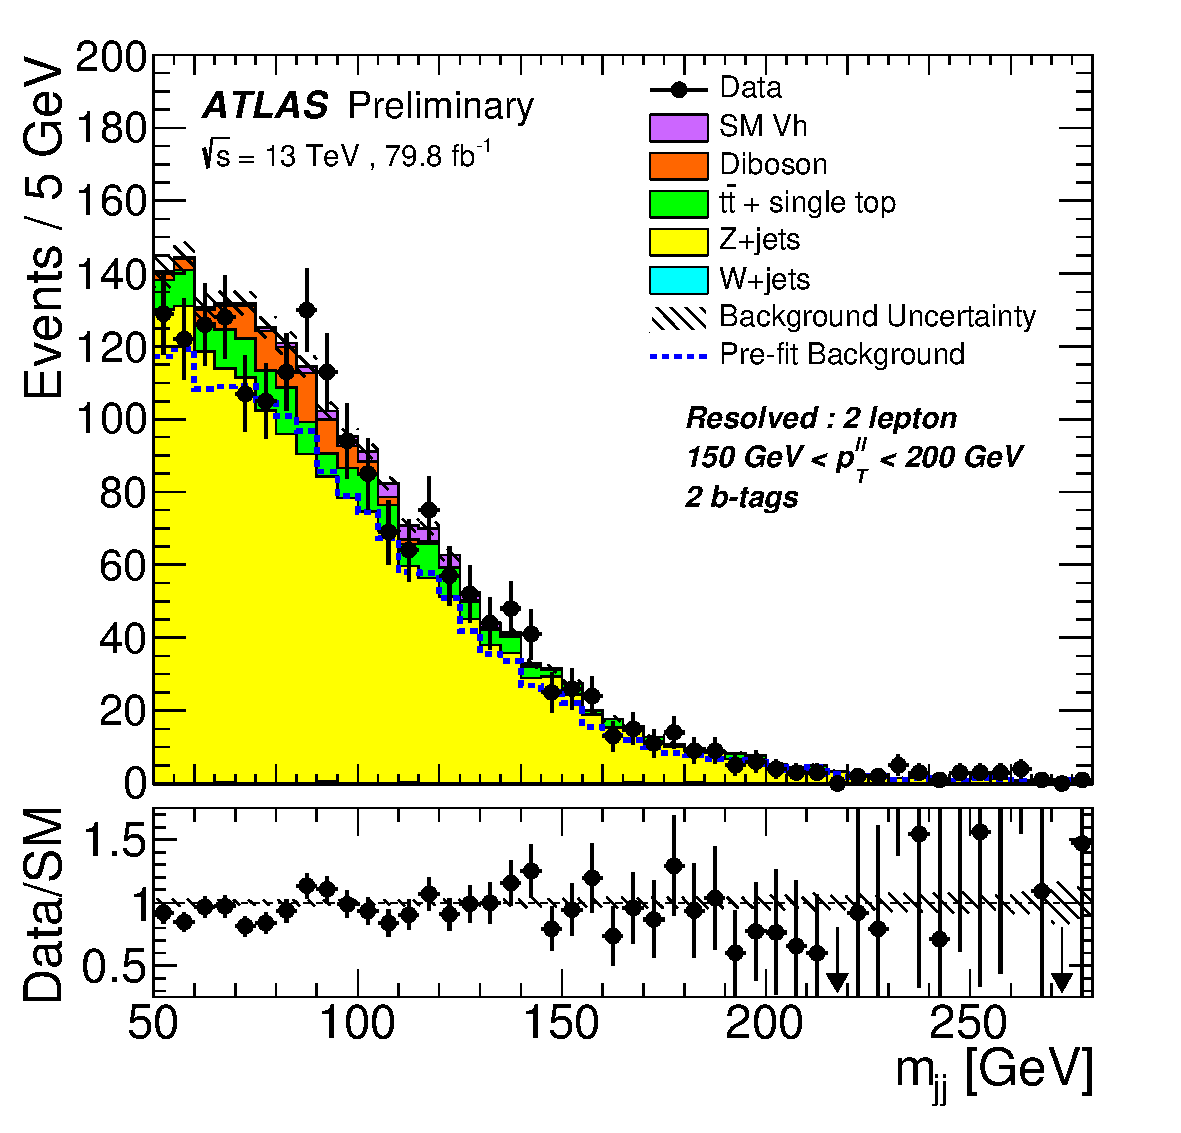
\includegraphics[width=0.47\linewidth]{postfit-150-200.pdf}}
	\subcaptionbox
	{$200\, \mathrm{GeV} < p^V_T < 350\, \mathrm{GeV}$
		\label{fig:2-lep-postfit-fig2}}
		{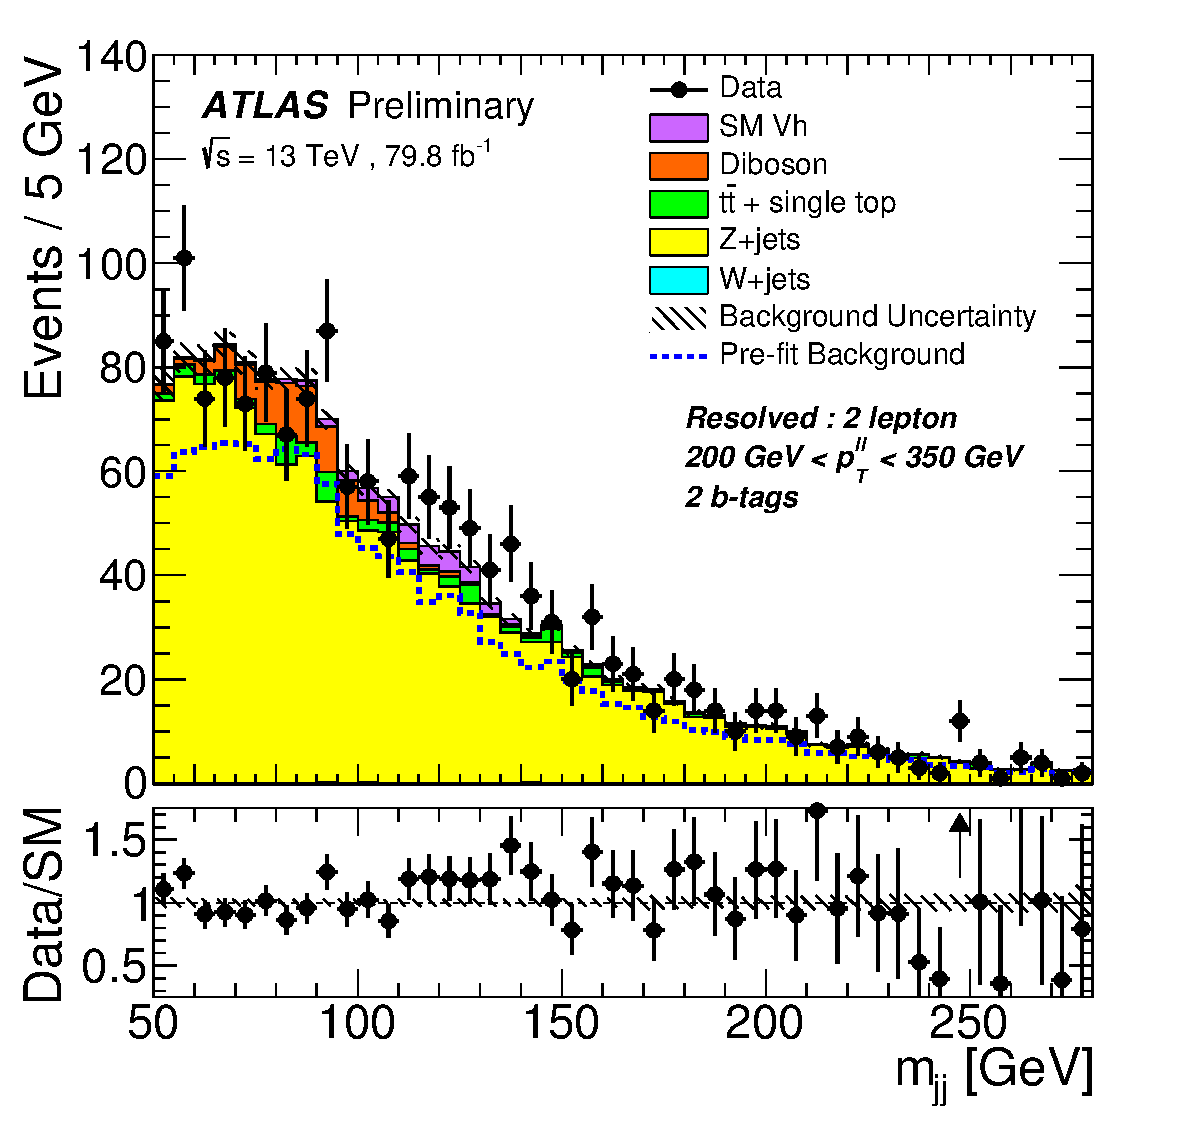
\includegraphics[width=0.47\linewidth]{postfit-200-350.pdf}}
	\vspace{\baselineskip}
	\subcaptionbox
	{$350\, \mathrm{GeV} < p^V_T < 500\, \mathrm{GeV}$
		\label{fig:2-lep-postfit-fig3}}
		{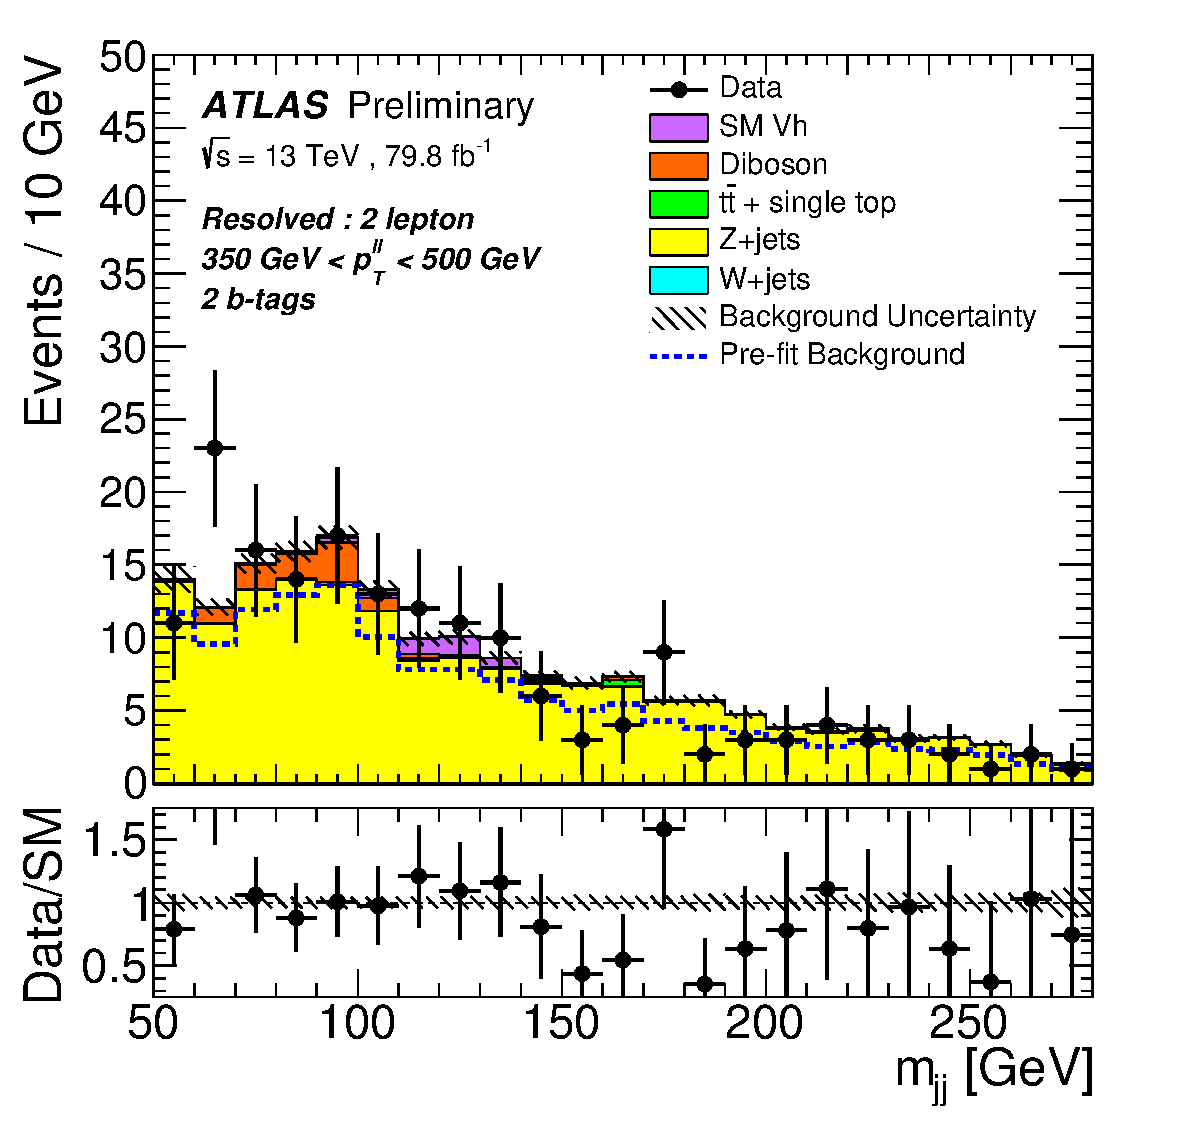
\includegraphics[width=0.47\linewidth]{postfit-350-500.pdf}}
	\subcaptionbox
	{$p^V_T > 500\, \mathrm{GeV}$
		\label{fig:2-lep-postfit-fig4}}
		{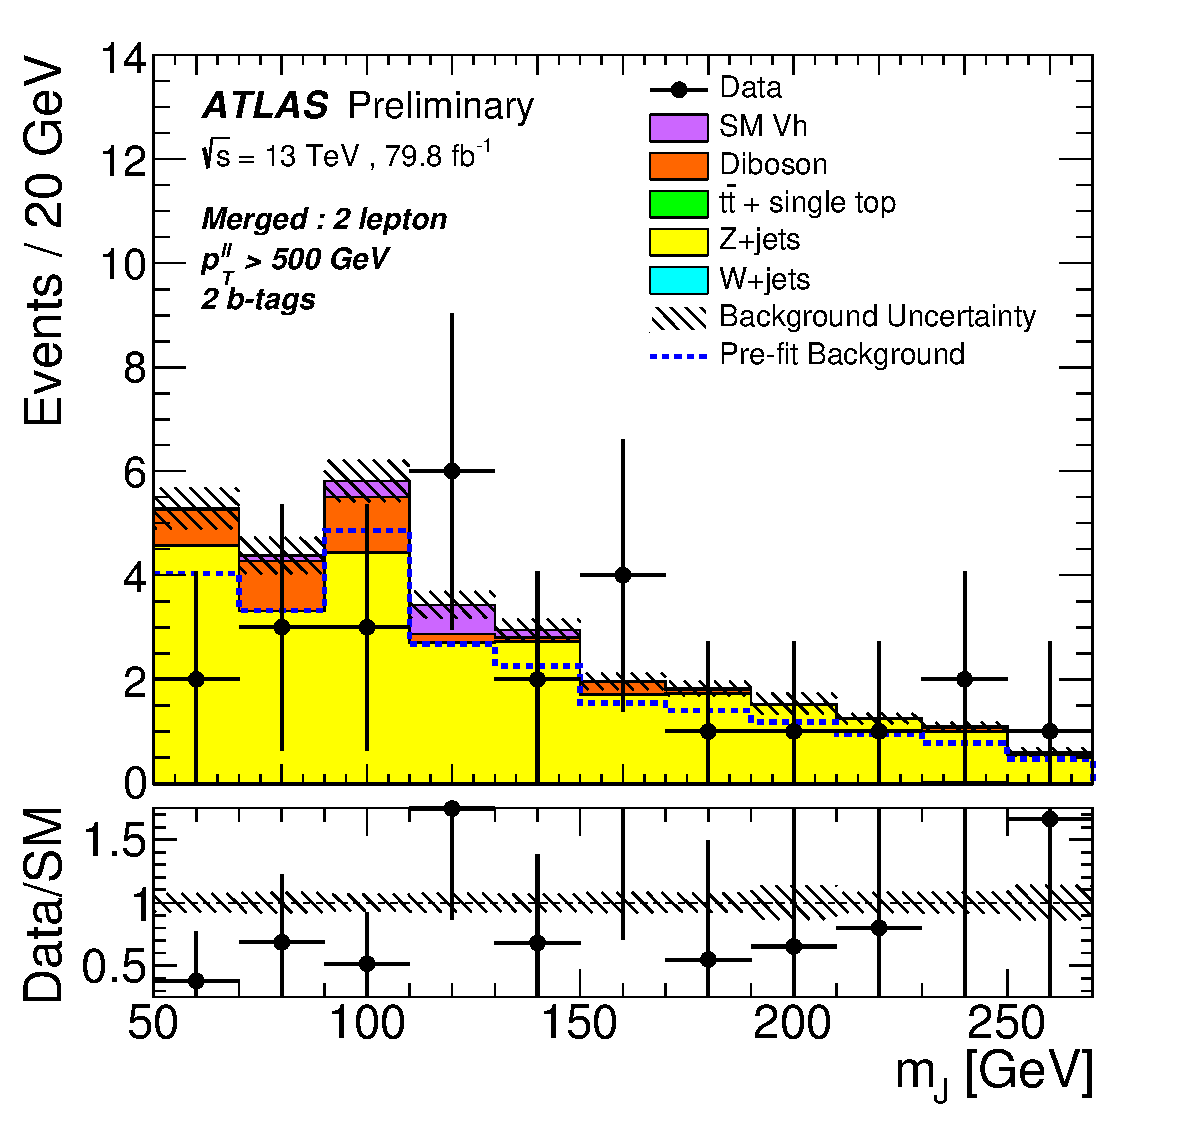
\includegraphics[width=0.47\linewidth]{postfit-500.pdf}}
	\caption{The post-fit data/MC comparison of $m_{bb}$ distribution. The plots are split into four $p^V_T$ regions for fitting.}
	\label{fig:2-lep-postfit}
\end{figure}

\end{document}
        \documentclass[class=NTHU_thesis, crop=false]{standalone}
\begin{document}

\chapter{The Results}
\label{chap:result}
The binned likelihood approach is used to get the final fitting result. The data are binned into four regions in $E^{miss}_T$ ($p^V_T$ in CR) to fit simultaneously, three for the resolved region, $[150\, \mathrm{GeV}, 200\, \mathrm{GeV})$, $[200\, \mathrm{GeV}, 350\, \mathrm{GeV})$ and $[350\, \mathrm{GeV}, 500\, \mathrm{GeV})$, and one for the merged region, $[500\, \mathrm{GeV}, \infty)$. For the SR, the mass of the Higgs boson candidate $m_h$ is the fit variable. For the background estimation, the charge of $\mu$ is used as the discriminating variable in one-muon CR to separate $W$($\mu\nu$) + jets and $t\bar{t}$. The $t\bar{t}$ is expected to have equivalent $\mu^+$ and $\mu^-$, while the $W$ + jets process is expected to have more $\mu^+$ than $\mu^-$. In the two-lepton CR, the total yield is used as the fit variable. The jets containing $b$- or $c$-quarks, expressed as heavy flavor jets (HF), dominate in the main background. The normalization of $Z$ + HF, $W$ + HF and $t\bar{t}$ is free parameters in the fit and the different flavor composition between the two jets, like $bb$, $bc$, $bl$ ($l$ for light quarks) and $cc$ provides the systematic uncertainties. The normalization factors of $Z$ + HF, $W$ + HF and $t\bar{t}$ are fitted to be $1.42 \pm 0.10$, $1.51 \pm 0.22$ and $1.10 \pm 0.08$, respectively. For the sub-dominant background, the MC simulation is constrained by theory prediction.

Thanks to the application of the VR track jets, the object-based $E^{miss}_T$ significance, as well as the increased luminosity, the result of the analysis becomes further improved, as shown in \cref{fig:VRvsFR}. The distribution of $E^{miss}_T$ for the SR, including the resolved region and merged region combined, is shown in \cref{fig:result-MET-mass} and no significant excess is observed. The results are further interpreted as exclusion limits at 95\% confidence level (CL). The exclusion contour of the $Z^\prime$-2HDM parameters $(m_{Z^\prime}, m_A)$ is depicted in \cref{fig:result-limit} and the observation is consistent with the expectation\cite{ATLAS-CONF-2018-039}.

\fig[0.65][fig:VRvsFR][!hbt]{VRvsFR.pdf}[The comparison of the expected upper limit on the signal strength between the analysis with VR track jets and the previous iteration of the analysis with FR track jets. Other differences between the two analyses also include the application of the object-based $E^{miss}_T$. Obvious improvement is shown in the high $m_{Z^\prime}$ region.]

\fig[0.65][fig:result-MET-mass][!hbt]{result-MET-mass.pdf}[The distribution of $E^{miss}_T$ for the SR, including the resolved region and merged region combined. The solid histogram and the blue dashed line in the upper panel present the comparison between the data and the SM prediction after and before the fit, respectively. The expected $Z^\prime$-2HDM signal is also shown by the red dashed line. The lower panel shows the ratio of the data to the post-fit SM prediction. No significant excess is observed.]

\fig[0.65][fig:result-limit][!hbt]{result-limit.pdf}[The exclusion contour of the $Z^\prime$-2HDM parameters $(m_{Z^\prime}, m_A)$ for other fixed parameter value, $tan(\beta) = 1$, $g_Z = 0.8$ and $m_\chi = 100\, \mathrm{GeV}$. The observation is consistent with the expectation within the uncertainty. The previous ATLAS result is also shown.]

\end{document}      % 結論
        % \documentclass[class=NTHU_thesis, crop=false]{standalone}
\begin{document}

\chapter{Chapter name(demo)}
Content of chapter \\
Content Content Content.

\section{Section name}
Content of section \\
Content Content Content
\subsection{Subsection name}
Content of subsection \\
Content Content Content

\subsubsection{Subsubsection name}
Content of subsubsection \\
Content Content Content

\paragraph{Paragraph name}
Content of paragraph \\
Content Content Content

\subparagraph{Subparagraph name}
Content of subparagraph \\
Content Content Content


\chapter{Test demo}
First line.
(next line in \LaTeX\ )still first line. \\
Second line.


\chapter{figure}
\section{Insert single figure(by sppmg's tool)}
\fig[0.15][fig:label_test][!hbt]{logo-Linux.png}[caption][short caption]

\section{Insert figures}
\begin{figure}[!hbt]
    %\captionsetup[subfigure]{labelformat=empty} % hide figure's number.
    \centering
    \subcaptionbox
        {caption\_1
        \label{fig:subfig_fig1}}
        {
\includegraphics[width=0.3\linewidth]{fig1.png}}
    ~
    \subcaptionbox
        {caption\_2
        \label{fig:subfig_fig2}}
        {
\includegraphics[width=0.3\linewidth]{fig2.eps}}
    \vspace{\baselineskip} % 分隔上下列
    \subcaptionbox
        {caption\_3
        \label{fig:subfig_fig3}}
        {
\includegraphics[width=0.6\linewidth]{fig3.png}}
    \caption{caption, use ``\subref{fig:subfig_fig2}'' get ID of subfigure(this ID is Debian) in caption}
    \label{fig:label}
\end{figure}


\chapter{Table}
\section{Simple table}
\begin{table}[h]
    \centering
    \caption{Solution}
    \begin{tabular}{| l | l |}
        \hline
        Component  & Concentration(mM) \\ \hline
        \ce{CaCl2} & 118.0 \\ \hline
    \end{tabular}
\end{table}

\section{Auto break line table}
\begin{table}[h]
    \centering
    \begin{tabularx}{\textwidth}{| l | X |}
        \hline
        short & short short \\ \hline
        long  & long long long long long long long long long long \\ \hline
    \end{tabularx}
\end{table}

\end{document}
    \backmatter          % book class 預設\backmatter 在\appendix 後面。因此.cls修改過\appendix 定義
        % This file has 3 types bibliography management, 
% \bibManType in config.tex choose it.
% 0. Embedded: write \bibitem in {thebibliography} environment.
% 1. BibTeX: Change bib files in \bibliography{}
% 2. biber / BibLaTeX: Add bibliography by \addbibresource{bibfile.bib} in macros_preamble.tex

\documentclass[class=NTHU_thesis, crop=false]{standalone}

\begin{document}

\ifcase \bibManType 
    % 0 == Embedded %%%%%%%%%%%%%%%%%%%%%%%%%%%%%%%%%%%%%%%
    {\bibFontStyle\setstretch{\bibLineStretch}
    \begin{thebibliography}{99}

    \bibitem{cite_key_1}
        bibliography item detail.

    \bibitem{_sppmg/tw_thesis_template_????}
        TW\_Thesis\_Template,
        sppmg,
        \url{https://github.com/sppmg/TW_Thesis_Template},
        Embedded bibliography demo.

    \end{thebibliography}
    }
    
\or
    % 1 == BibTeX %%%%%%%%%%%%%%%%%%%%%%%%%%%%%%%%%%%%%%%%%
    \bibliographystyle{\bibStyle}
    {\bibFontStyle\setstretch{\bibLineStretch}
        \bibliography{demo} % {sample_1,sample_2,...,sample_n}
        % Note the lack of whitespace between the commas and the next bib file.
    }
\or

    % 2 == biber / BibLaTeX %%%%%%%%%%%%%%%%%%%%%%%%%%%%%%%
    \printbibliography[heading = bibnumbered, title = {Reference}]
\fi



\end{document}
    \appendix
        \documentclass[class=NTHU_thesis, crop=false]{standalone}
\begin{document}

\chapter{List of device}

\begin{table}[!h]
    \centering
    \begin{tabularx}{\textwidth}{|l|l|X|}
        \hline
        device  & Model    & Description \\ \hline
        Linux   & Debian 9 & Best of best of best OS \\ \hline
        Windows & 10       & Best of Best tool to prevent the aging of brain. \\ \hline
    \end{tabularx}
    \caption{List of device}
    \label{table:list_device}
\end{table}

\end{document}
        \documentclass[class=NTHU_thesis, crop=false]{standalone}
\begin{document}

\definecolor{Gray3}{gray}{0.8}

\chapter{Solutions}

\section{The solution}
\begin{table}[!h]
    \centering
    \begin{tabular}{| l | l |}
        \hline
        Component & Concentration(mM) \\ \hline
        \rowcolor{Gray3}
        \ce{NaCl} & 1.0 \\ \hline
        \ce{CaCl_2} & 2.0 \\ \hline
        \rowcolor{Gray3}
        \ce{NaCl} & 1.0 \\ \hline
        \ce{CaCl_2} & 2.0 \\ \hline
    \end{tabular}
    \caption{The solution}
\end{table}
\end{document}
        \documentclass[class=NTHU_thesis, crop=false]{standalone}
\begin{document}
% Here demo instert whole code file. You can only insert code directly, 
% please read my tutorial or document of listings package.
% code style set in macros_preamble already.
% Supported language please read document of listings package.


\chapter{Code}
\section{C}
\lstinputlisting[language=C]{hello_world_c.c}

\section{Matlab}
\lstinputlisting[language=matlab]{hello_world_matlab.m}

\section{IDL}
\lstinputlisting[language=IDL]{hello_world_idl.pro}
\end{document}

%         \documentclass[class=NTHU_thesis, crop=false]{standalone}

\begin{document}
\chapter{Letters bot}

Here try to insert some information automatically.
If you need change font size or position, modify appendix\_letter\_NCU.tex and compile this single tex file.

In appendix\_letter\_NCU.tex, you will see \textbackslash{}placetextbox for every string.
\begin{lstlisting}[style=LatexStyle,caption={}]
\placetextbox{x(mm)}{y(mm)}
\end{lstlisting}

The unit is mm , origin at bottom left. I recommend add ``colorgrid'' option to ``\textbackslash{}documentclass'' for positioning. e.g. In this tex file (appendix\_letter\_NCU.tex):

\begin{lstlisting}[style=LatexStyle,caption={}]
\documentclass[class=NTHU_thesis, crop=false, colorgrid]{standalone}
\end{lstlisting}

``colorgrid'' will display a grid with mm unit. 

\begin{center}
{ \noindent\color{red}\bfseries\Large NCU 中文文件位於 NCU\_zh}
\end{center}

%%%%%%%%%%%%%%%%%%%%%%%%%%%%%%%%
% define \mprof 
\ExplSyntaxOn
    % Copy prof. list from config.tex
    \clist_gclear_new:N \g_sppmg_profs_cl
    \clist_gset:NV \g_sppmg_profs_cl \profs
    \clist_gpop:NNTF \g_sppmg_profs_cl \l_tmpa_tl {}{ \tl_clear:N \l_tmpa_tl}
    \cs_gset_eq:NN \mprof \l_tmpa_tl
\ExplSyntaxOff

% Define local variable (e.g. cover use \titleZh for \title but letters use \titleEn )
\def\title{\titleEn}

%%%%%%%%%%%%%%%%%%%%%%%%%%%%%%%%
\cleardoublepage
\pagestyle{empty}
\sffamily
% ------------------------------

% 碩博士論文電子檔授權書
\IfFileExists{\letterAuthEl}{
\cleardoublepage\thispagestyle{empty}
\includepdf[pagecommand={   \placetextbox{115}{87}{\fs{14}\title}%
                            \placetextbox{100}{81}{\fs{14}\mprof}%
                            \placetextbox{85}{70}{\fs{14}\deptshort} }]%
{\letterAuthEl}}{}

% 碩博士紙本論文延後公開/下架申請書。(如需延後公開者,才需要裝訂於論文內頁)
\IfFileExists{\letterPubReq}{
\cleardoublepage\thispagestyle{empty}
\includepdf[pagecommand={   \placetextbox{128}{269}{\fs{14}\author}%
                            \placetextbox{70}{255}{\fs{14}\deptshort}%
                            \placetextbox{100}{231}{\fs{14}\title}%
                            \placetextbox{90}{218.3}{\fs{14}\mprof} }]%
{\letterPubReq}}{}

% 指導教授推薦書
\IfFileExists{\letterRecom}{
\cleardoublepage\thispagestyle{empty}
\includepdf[pagecommand={   \placetextbox{75}{204}{\fs{16}\deptshort}%
                            \placetextbox{90}{218}{\fs{16}\author}%
                            \placetextbox{105}{192}{\fs{16}\title}}%
]{\letterRecom}}{}

% 口試委員審定書
\IfFileExists{\letterVerif}{
\cleardoublepage\thispagestyle{empty}
\includepdf[pagecommand={   \placetextbox{75}{184}{\fs{16}\deptshort}%
                            \placetextbox{91}{200}{\fs{16}\author}%
                            \placetextbox{100}{170}{\fs{16}\title}}%
]{\letterVerif}}{}

% ------------------------------
\pagestyle{fancy}
\end{document}
\end{document}